% This is samplepaper.tex, a sample chapter demonstrating the
% LLNCS macro package for Springer Computer Science proceedings;
% Version 2.21 of 2022/01/12
%
\documentclass[runningheads]{llncs}


\usepackage{graphicx}
\usepackage{amssymb}
\usepackage{amsmath}
\usepackage{stmaryrd}
\usepackage[hyphens]{url}
\usepackage[inline]{enumitem}
\usepackage{hyperref}
\usepackage{listings}
\usepackage{color}
\usepackage{myacronyms}
\usepackage{booktabs}
\usepackage{subcaption}
\usepackage{xspace}
\usepackage{cleveref} % import this as the last one!
\usepackage{./code-listings}
\usepackage{todonotes}

\newcommand{\sidenote}[3]{\todo[linecolor=#1,backgroundcolor=#1!25,bordercolor=#1,size=\tiny]{\textbf{#2:} #3}}
\renewcommand{\note}[3]{\todo[inline,linecolor=#1,backgroundcolor=#1!25,bordercolor=#1]{\textbf{#2:} #3}}

\newcommand{\aonote}[1]{\note{red}{AO}{#1}}
\newcommand{\aosidenote}[1]{\sidenote{red}{AO}{#1}}

\newcommand{\malanote}[1]{\note{violet}{Mattia}{#1}}
\newcommand{\malasidenote}[1]{\sidenote{violet}{Mattia}{#1}}

\newcommand{\mmnote}[1]{\note{yellow}{Matteo}{#1}}
\newcommand{\mmsidenote}[1]{\sidenote{yellow}{Matteo}{#1}}

\newcommand{\teonote}[1]{\note{cyan}{Teo}{#1}}
\newcommand{\teosidenote}[1]{\sidenote{cyan}{Teo}{#1}}

\newcommand{\gcnote}[1]{\note{green}{Gio}{#1}}
\newcommand{\gcsidenote}[1]{\sidenote{green}{Gio}{#1}}

\newcommand{\missingref}[1][{add some ref here}]{\sidenote{orange}{TODO}{#1}}

% Custom environments
\newenvironment{inlinelist}{\begin{enumerate*}[label=\emph{(\roman*)}]}{\end{enumerate*}}

%%%%%%% FIX CLEVEREF/ACRONYM https://tex.stackexchange.com/questions/735500/% problem-with-amsmath-cleveref-acronym
\makeatletter
\AtBeginDocument
 {
   \def\ltx@label#1{\cref@label{#1}}%add braces
   \def\label@in@display@noarg#1{\cref@old@label@in@display{#1}}%remove braces
\def\label@in@mmeasure@noarg#1{%
    \begingroup%
      \measuring@false%
      \cref@old@label@in@display{#1}%remove braces for multline, see https://% tex.stackexchange.com/q/737204/2388
    \endgroup}%
 } %
\makeatother
%%%%%%% END FIX CLEVEREF/ACRONYM

\newcommand{\ourapproach}[0]{\textsc{AGE-ML}}


\begin{document}
\sloppy
%
\title{Agentic Architecture for Data-Centric \acs{AutoML}}
%
%\titlerunning{Abbreviated paper title}
% If the paper title is too long for the running head, you can set
% an abbreviated paper title here
%
\author{
Mattia Matteini\inst{1}\orcidID{0009-0007-4474-8431} \and
Matteo Magnini\inst{2}\orcidID{0000-0001-9990-420X} \and
Matteo Francia\inst{1}\orcidID{0000-0002-0805-1051} \and
Giovanni Ciatto\inst{1}\orcidID{0000-0002-1841-8996} \and
Andrea Omicini\inst{1}\orcidID{0000-0002-6655-3869}
}
%
\authorrunning{M. Matteini et al.}
% First names are abbreviated in the running head.
% If there are more than two authors, 'et al.' is used.
%
\institute{Department of Computer Science and Engineering, Alma Mater Studiorum---Universit\`a di Bologna, Cesena, Italy\\
\email{\{mattia.matteini,m.francia,giovanni.ciatto,andrea.omicini\}@unibo.it} \and
Department of Computer Science, Faculty of Science, Technology and Medicine, University of Luxembourg, Esch sur Alzette, Luxembourg\\
\email{matteo.magnini@uni.lu}}
%
\maketitle              % typeset the header of the contribution
%
\begin{abstract}
Data-Centric \ac{AI} focuses on improving data quality and curation as the main driver of machine learning performance.
%
Although \ac{AutoML} has reduced the cost of model selection and hyperparameter tuning,
most systems remain model-centric and poorly aligned with \ac{MLOps} requirements such as controllability, traceability, and explainability: automated choices about preprocessing, pipeline structure, and validation are often opaque and difficult to revise, despite their strong influence on model behaviour.
%
We propose \ourapproach{}, a specification-driven, \textit{agentic} architecture for Data-Centric AI.
%
A human-readable specification language enables data scientists to encode assumptions, constraints, evaluation criteria, and design preferences across the pipeline.
%
\acp{LLM} operate within a controlled agent loop to interpret specifications, generate and validate execution plans, synthesize pipeline code, and produce structured explanations.
%
Algorithmic optimization remains separate from \ac{LLM}-based reasoning to ensure reproducibility and controlled automation.
%
Results show improved transparency, iterative pipeline refinement, and stronger integration with \ac{MLOps} practices such as experiment tracking and reproducibility.
%
Finally, we discuss limitations and future directions for \ourapproach{}.

\keywords{MLOps \and
Data-centric AI\and
Agentic AI\and
AutoML\and
LLMs}
\end{abstract}
%
%
%

\begin{figure*}%[t]
  \centering
  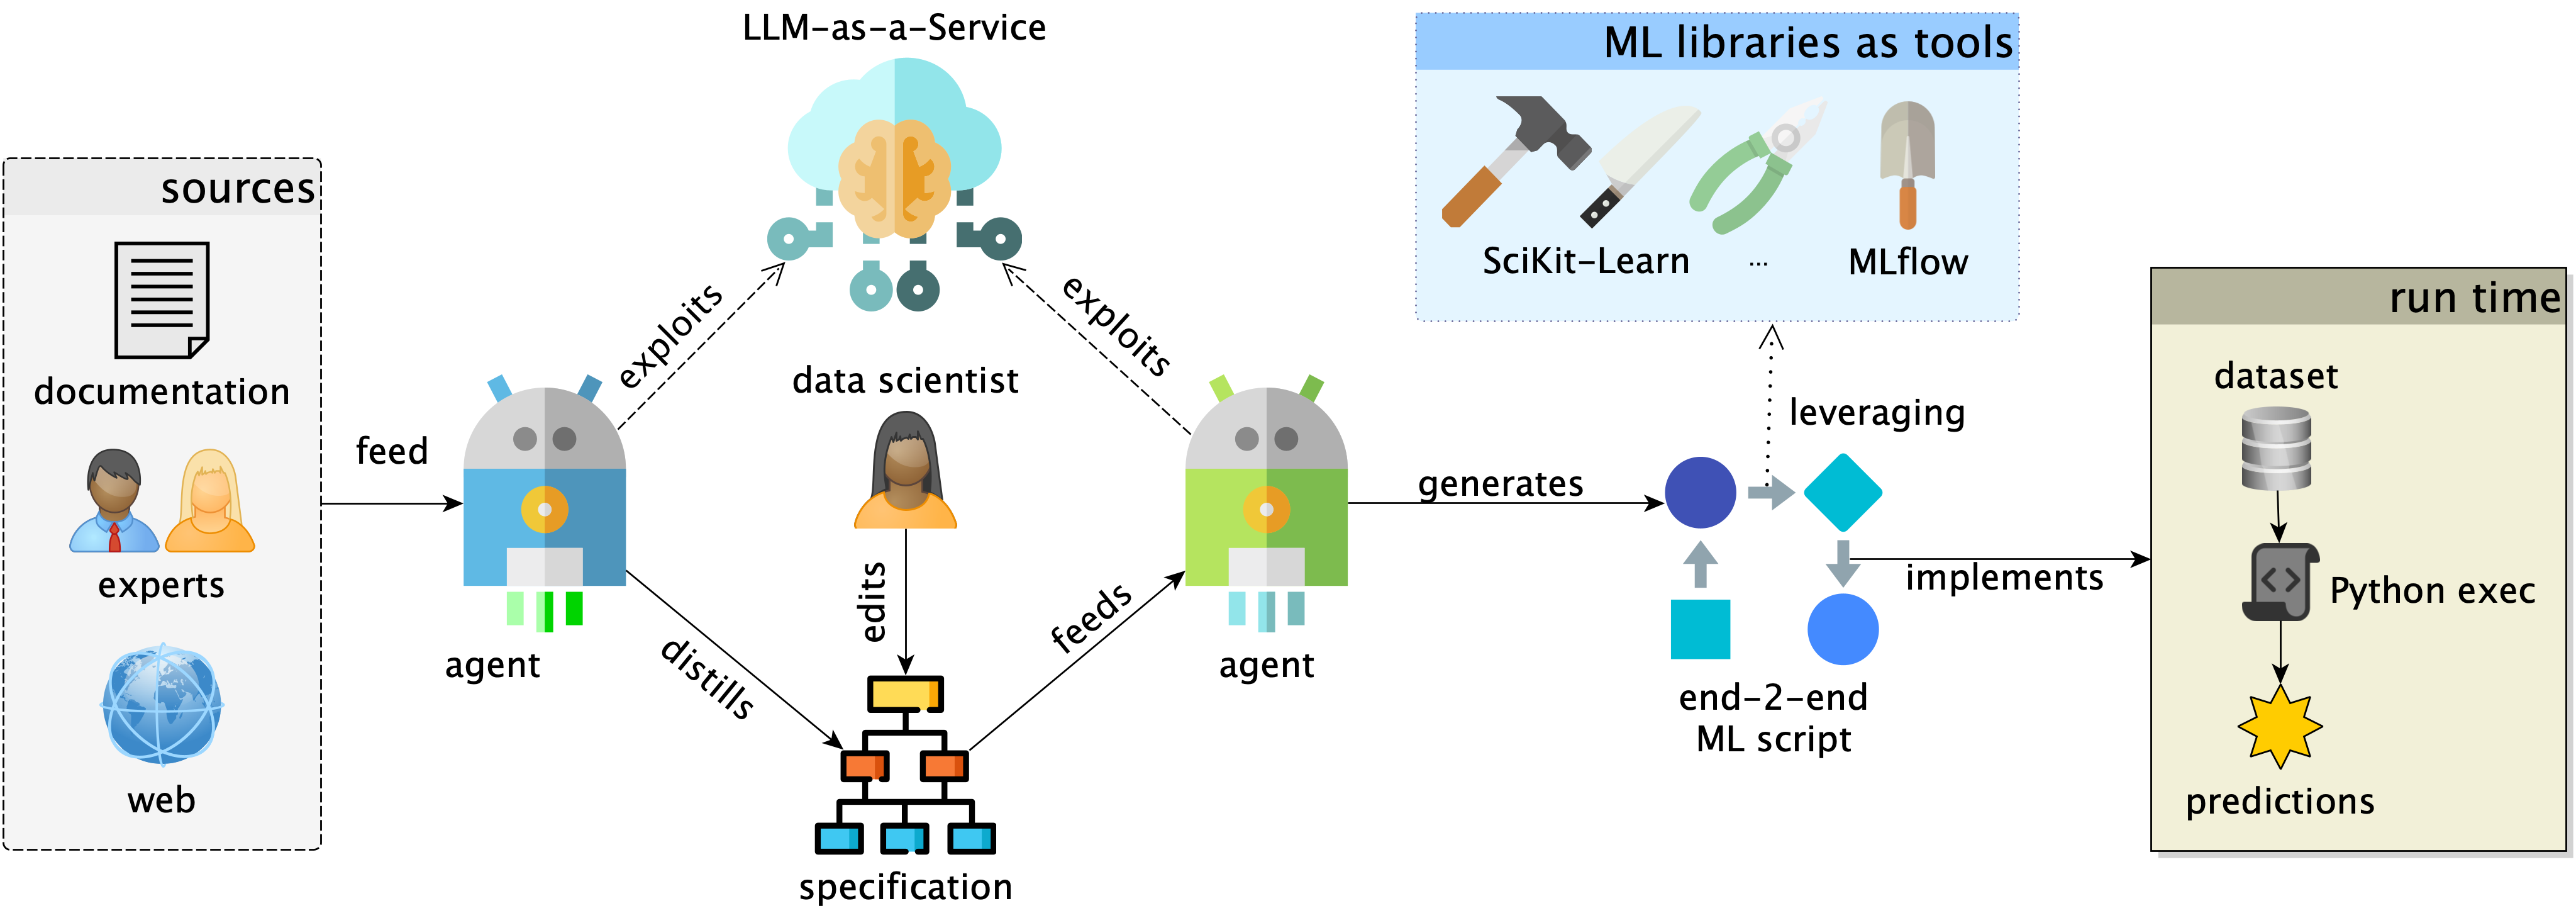
\includegraphics[width=\linewidth]{figures/agentic-automl-research-line.png}
  \caption{
    % \emph{Research line overview:}
    %
    \ourapproach{}: data scientists encode their \ac{ML} knowledge in a structured specification.
    %
    Then, it lets
    agents (green) generate end-to-end \ac{ML} code leveraging well-known \ac{ML} libraries as tools.
    %
    \Acp{LLM} are exploited as a service by agents in order to generate code and reason about the data.
    %
    Generated code is automatically run on actual datasets to produce predictions.
    %
    % \emph{Future work:}
    % (currently not supported by \ourapproach{})
    % the specification will be generated by agents (blue) as well,
    % based on various sources, such as written documentation, internet resources, or conversations with domain experts.
  }
  \label{fig:research-line}
\end{figure*}

\section{Introduction}

Data-centric \ac{AI} emphasises the improvement of data quality and curation as the primary driver of the performance of machine learning models~\cite{zha2025data}.
%
In this paradigm,
the role of the data scientist extends beyond model selection and hyperparameter tuning to the design of effective data preprocessing, feature engineering, and validation.
%
Injecting domain and a-priori experience into \ac{ML} pipelines is therefore essential.
%
However,
modern \ac{ML} systems are characterised by a fundamental duality between integrating human expertise and automation.
%
On one hand,
data scientists possess domain knowledge,
a-priori experience,
and contextual understanding
that are indispensable for designing robust and trustworthy pipelines~\cite{DBLP:conf/pakdd/FranciaGG24}.
%
On the other hand,
the increasing scale and velocity of data demand \emph{automation} to ensure efficiency, reproducibility, and scalability~\cite{he2021automl}.

In such automation,
our perspective is to reposition human effort toward high-value tasks
(as observed in practices such as vibe coding~\cite{welsh2022end})
rather than low-level coding,
repetitive experimentation,
and manual orchestration of workflow components;
all of which are tasks that could be automated by coding frameworks
(such as \texttt{MLflow}~\cite{zaharia2018accelerating} and \texttt{auto-scikit-learn}~\cite{DBLP:journals/jmlr/FeurerEFLH22} pipelines).
%
Automation should act as an amplifier of expertise,
handling execution and optimisation while preserving meaningful human control over the structure and logic of the pipeline.
%
Despite their empirical effectiveness, many \ac{AutoML} systems~\cite{zha2025data} exhibit a mismatch with data-centric \ac{AI} principles.
%
Traditional \ac{AutoML} approaches primarily concentrate on model selection and hyperparameter optimisation,
often treating the dataset as fixed and immutable.
%
While this strategy can yield strong benchmark results,
it overlooks the iterative and data-focused processes that characterise real-world machine learning practice and the well-established principles of CRISP-DM~\cite{schroer2021systematic}.

% Purely optimisation-driven \ac{AutoML} systems may violate the semantics of features,
% or hide critical choices from the data scientist;
% also, they are not flexible enough to integrate user feedback.
% %
% As a result,
% there exists a conceptual and practical gap between the optimisation-centric view of \ac{AutoML} and the knowledge-driven, data-first philosophy of data-centric \ac{AI}.

% \paragraph{Contribution}

In this paper we propose \ourapproach{}, an \emph{agentic} architecture for automatic \emph{end-to-end} pipeline generation and execution that aligns with data-centric \ac{AI} principles.
%
Thanks to \ac{LLM}-based intelligent agents, \ourapproach{}
\begin{inlinelist}
    \item enables structured integration of expert knowledge into automated processes
    (e.g., via natural language),
    %
    \item it reduces operational load for data scientists
    (by automating generation and execution of low-level coding and tuning tasks),
    %
    and
    %
    \item it supports modularity and reusability of knowledge
    (data scientists' knowledge can be encoded, extended, and shared over time).
\end{inlinelist}
\ourapproach{}
(\cref{fig:research-line})
delegates \ac{ML} pipelines' design and implementation to a \ac{MAS} where agents interleave
symbolic reasoning,
intuitive reasoning and text generation
(as provided by \acp{LLM}),
and execution of generated code
to automatise and explain \ac{ML} operations.
%
Crucially,
\ourapproach{} enables structured human knowledge injection during pipeline creation,
via an \emph{ad-hoc} specification language.
%
Domain experts can constrain search spaces,
define preferred preprocessing strategies,
or
embed domain rules directly into their specification file.
%
This paradigm combines automated optimisation of AutoML with guided expertise,
producing pipelines that are not only performant but also inspectable, explainable, adaptable,
and aligned with domain requirements.



The remainder of the paper is organised as follows.
\cref{sec:background-and-motivation} provides background on data-centric \ac{AI}, \ac{AutoML}, and agentic \ac{AI}.
\cref{sec:agentic-architecture-for-specification-driven-automl} introduces the architecture of \ourapproach{} and \cref{sec:experimental-evaluation} evaluates it also against state-of-the-art approaches.
\cref{sec:conclusion} concludes the paper also with a discussion on future works.

\section{Related Works}
\label{sec:background-and-motivation}

Data-centric \ac{AI} prioritises improving data quality and representativeness over focusing primarily on \ac{ML} models~\cite{zha2025data}.
%
It shifts the main optimisation target from model design to data quality,
treating high-quality data as a powerful lever for improving system performance.
%
For example,
consider a classification task predicting loan approval/denial.
%
Suppose a \ac{DT} classifier is trained on past application data.
%
In a \emph{model}-centric approach,
if the \ac{DT} yields unsatisfactory accuracy,
we might increase its depth,
try random forests,
switch to gradient boosting,
or tune hyperparameters,
so to increase accuracy.
%
In a \emph{data}-centric approach,
we keep the \ac{DT} fixed and inspect the dataset instead.
%
There we may spot data quality issues,
e.g. mislabeled examples,
or distributional biases.
%
After correcting these issues via ad-hoc data cleaning, %and retraining the same decision tree,
%performance could improve because the training data would better reflect the true decision patterns.
re-training the same \ac{DT} (i.e., with the same hyper-parameters) may yield better performance.

In this context, \Ac{AutoML} reduces the manual effort of building and tuning \ac{ML} models by automating parts of the development process.
%
However, most approaches focus primarily on \ac{HPO} and model selection,
improving predictive performance through the exploration of model families, preprocessing strategies, and hyperparameters.
%
While effective, this remains largely model-centric and does not explicitly address reproducibility, auditability, or controllability across the broader \ac{ML} lifecycle.
%
Moreover, \ac{AutoML} rarely incorporates knowledge about data semantics, provenance, or quality,
often treating datasets as static and reliable inputs.
%
As a result, it struggles to support data-centric refinement and reasoning about the suitability of the data itself.
%
Existing \ac{AutoML} systems rely on structured algorithmic search spaces,
which provide reproducibility and computational efficiency.
%
%However, they still require significant expert configuration and offer limited customisability.
%Several frameworks have been proposed,
%but many only focus on the modeling step of the \ac{ML} pipeline~\cite{he2021automl}.
%
TPOT~\cite{olson2016tpot},
Auto-WEKA~\cite{DBLP:conf/kdd/ThorntonHHL13},
and
Auto-Sklearn~\cite{DBLP:journals/jmlr/FeurerEFLH22}
are built on top of the \ac{CASH} problem,
which extends both the `Algorithm selection' problem
and
the \ac{HPO},
by searching for the best algorithm and also its hyperparameters for a given dataset.
%
Other frameworks
(e.g., Auto-Keras~\cite{DBLP:conf/kdd/JinSH19})
focus more on searching for deep learning models and support multi-modal and multi-task.
%
More recently,
FLAML~\cite{DBLP:conf/kdd/0001W0Q22} has outperformed the above-mentioned approaches.
%
Newer \ac{AutoML} frameworks also focus on end-to-end automation,
such as~\cite{FranciaGP23} and~\cite{DBLP:conf/pakdd/FranciaGG24}
which formalised and introduced \ac{AutoML} for end-to-end pipelines.


Other recent frameworks address end-to-end machine learning pipelines through \ac{LLM}-driven and multi-agent approaches.
%
DS-Agent~\cite{DBLP:conf/icml/GuoD0C0024} leverages case-based reasoning~\cite{kolodner1992introduction}
to iteratively construct and refine pipelines by retrieving and adapting prior solutions,
incorporating human insights
(e.g., from Kaggle)
and execution feedback.
%
CBR operates by retrieving similar past problems,
reusing their solutions for the current problem,
evaluating the effectiveness,
revising the solution,
and
retaining successful solutions.
%
MLZero \cite{DBLP:journals/corr/abs-2505-13941} extends this paradigm with a multi-agent architecture
that combines perception, semantic memory, and episodic memory
to iteratively generate, evaluate, and improve code,
enabling both domain knowledge integration and error-driven learning.
%
The semantic memory enhances the \ac{LLM}'s parametric knowledge with domain-specific information
from external knowledge that is not constructed by humans but rather by the summarisation agent
% (compresses relevant knowledge into concise paragraphs serving as queryable indices)
and the condensation agent.
% (transforms this knowledge into precise and streamlined guidance).
%
Similarly,
AutoML-Agent~\cite{DBLP:conf/icml/TriratJH25} adopts a coordinated multi-agent strategy to automate the full pipeline,
from data processing and model selection to deployment,
by decomposing the task into specialised roles.

Despite these advances,
current approaches still exhibit key limitations,
particularly in the lack of transparent optimisation processes and insufficient integration of constraints and domain semantics from data scientists,
motivating the need for more explainable and data-centric \ac{AutoML} solutions.
%
A detailed comparison of older contributions can be found in \cite{DBLP:conf/icml/TriratJH25}.

\paragraph{Distinguishing features of \ourapproach{}}

% % !TEX root = paper-2026-agentic-automl.tex

\newcommand{\Yes}{{\color{green}\checkmark}}
\newcommand{\No}{{\color{red}$\times$}}

\begin{table*}[t]
\centering
\scriptsize
\begin{tabular}{l|cc|cccc}
\hline
& \multicolumn{2}{c}{Non-LLM-based} 
& \multicolumn{3}{c}{LLM-based} \\
\cmidrule(lr){2-3} \cmidrule(lr){4-7}
Feature
                        & HAMLET \cite{FranciaGP23} & FLAML~\cite{DBLP:conf/kdd/0001W0Q22} & DS-Agent \cite{DBLP:conf/icml/GuoD0C0024} & AutoML-Agent \cite{DBLP:conf/icml/TriratJH25} & MLZero \cite{DBLP:journals/corr/abs-2505-13941} & \ourapproach \\
\hline
End-to-end pipeline     & \Yes                                           & \No                                  & \Yes                                       & \Yes                                           & \Yes                         & \Yes \\
Human-centered design   & \Yes                                           & \No                                  & \No                                        & \No                                            & \No                          & \Yes \\
Constrained generation  & \Yes                                           & \Yes                                 & \No                                        & \No                                            & \No                          & \Yes \\
Pipeline validation     & \Yes                                           & \No                                  & \Yes                                       & \Yes                                           & \Yes                         & \Yes \\
Interpretable pipeline  & \No                                            & \No                                  & \Yes                                       & \Yes                                           & \Yes                         & \Yes \\
Zero-data cold start    & \Yes                                           & \Yes                                 & \No                                        & \No                                            & \No                          & \Yes \\
MLOps oriented          & \No                                            & \No                                  & \No                                        & \No                                            & \No                          & \Yes \\
\hline
\end{tabular}
\caption{
    Comparison of recent \ac{AutoML} non-\ac{LLM} and \ac{LLM}-based approaches.
}
\label{tbl:automl_papers}
\end{table*}

% \cref{tbl:automl_papers} highlights the distinguishing characteristics of recent \ac{AutoML} approaches,
% positioning \ourapproach{} with respect to both non-\ac{LLM} and \ac{LLM}-based frameworks.
%
Non-\ac{LLM} approaches such as HAMLET and FLAML provide constrained generation and hot-start capabilities,
although only HAMLET supports end-to-end automation with a largely black-box optimisation process.
%
Existing \ac{LLM}-based systems enable flexible end-to-end pipeline construction and often include validation mechanisms,
but they typically lack explicit constraints, reducing reliability and reproducibility.
%
Moreover, data scientists usually provide only the initial task specification,
with limited involvement in later optimisation and refinement stages,
while resulting pipelines are often neither interpretable nor searchable.

% In this context, 
\ourapproach{} combines the strengths of both paradigms.
%
Unlike prior \ac{LLM}-based methods,
it introduces \emph{constrained generation} to improve robustness and enforce well-defined rules,
while preserving full end-to-end automation and integrating \emph{human-centred design}.
%
It also supports \emph{interpretable pipelines},
\emph{pipeline validation},
and \emph{searchability} through the data catalog.
%
Finally, its \emph{zero-data cold start capabilities} enable reuse of prior knowledge when available,
while still supporting adoption through default specifications alone.


% \section{Problem Statement and Formalisation}
% \label{sec:problem-statement-and-assumptions}

% \ac{ML} workflows are commonly described as sequential pipelines from data provisioning to model training, validation, and deployment.
% %
% In practice,
% however,
% their construction involves iterative and interdependent activities such as
% data cleaning and transformation,
% augmentation,
% feature engineering,
% model selection,
% hyperparameter tuning, and
% cross-validation.
% %, and sometimes ensembling.
% %
% The decisions taken in one phase affect the others:
% for instance,
% feature engineering depends on the models under consideration,
% whereas model selection depends on which transformations are feasible or beneficial for the available data.

% A central difficulty is that much of the knowledge required to conduct such workflows remains implicit
% in textbooks, tools, or experts' experience.
% %
% This limits
% \begin{inlinelist}
%   \item automation, because tacit heuristics cannot be directly executed;
%   \item explanation, because the rationale behind workflow decisions is rarely recorded;
%   and
%   \item reproducibility, because the process that produced a model is difficult to reconstruct.
% \end{inlinelist}
% %
% Although \ac{AutoML} has substantially advanced algorithm selection and hyperparameter tuning,
% and \ac{MLOps} has improved orchestration, traceability, and lifecycle management,
% neither perspective fully supports the explicit representation, execution, and explanation of data-science knowledge across the whole workflow.
% %
% We therefore address three problems:
% %
% \begin{enumerate*}[label=(\textbf{P\arabic*})]
%     \item\label{prob:knowledge-encoding}provide data scientists with a way to express their data-science knowledge; % in a human- and machine-interpretable form;
%     %
%     \item\label{prob:workflow-automation}leverage such knowledge to automate the execution of the whole \ac{ML} workflow; %, not just isolated sub-tasks;
%     %
%     \item\label{prob:explanation}trace and explain the sequence of decisions that leads %from a dataset and a predictive goal
%     to a satisfactory model selection.
% \end{enumerate*}

% Problem \ref{prob:knowledge-encoding} concerns the design of a language that is both human- and machine-interpretable.
% %
% Such a language should let practitioners specify and revise:
% %
% \begin{inlinelist}
%     \item the admissible workflow steps and their ordering,
%     e.g., preprocessing $\rightarrow$ feature engineering $\rightarrow$ model selection $\rightarrow$ training;
%     %
%     \item the algorithms or procedures implementing each step,
%     e.g., missing-value imputation, one-hot encoding, or model families;
%     %
%     \item the corresponding hyperparameters,
%     e.g., imputation strategy or the value of $k$ in $k$-NN;
%     %
%     \item the conditions under which choices are required, forbidden, or preferable,
%     e.g., imputation is required only when missing values occur,
%     whereas one-hot encoding is relevant only for categorical features and models requiring numerical inputs.
% \end{inlinelist}

% Problem \ref{prob:workflow-automation} concerns the execution of workflows defined by such specifications.
% %
% Given a dataset and a predictive goal,
% the system should determine which steps to perform,
% which algorithms to instantiate,
% and which hyperparameters to select.
% %
% Operationally,
% the workflow is a computational process that takes an \ac{ML} problem instance as input and returns a trained model together with the artefacts required for evaluation and deployment.
% %
% In this work,
% we focus on supervised predictive tasks where the target variable is already present in the dataset:
% classification when the target is categorical,
% and regression when it is numerical.

% Problem \ref{prob:explanation} concerns the intelligibility of automated decisions.
% %
% The system should not only return a model,
% but also record and summarise the decisions leading to it.
% %
% This includes,
% for example,
% why a task was treated as classification or regression,
% why a preprocessing step was enabled or inhibited,
% why a model family was explored,
% and how data evidence or intermediate evaluation results affected later choices.
% %
% The resulting explanation should let users assess the correctness, completeness, and practical adequacy of the generated workflow.

% \subsection{Research Line Overview}
% \label{subsec:overview-of-the-research-line}

% \cref{fig:research-line} summarises the research line through which we address the problems above and,
% in the longer term,
% the broader vision of data-centric \ac{AutoML}.

% The core element is an explicit \emph{specification}
% encoding methodological knowledge about \ac{ML} workflows,
% thereby addressing problem \ref{prob:knowledge-encoding}.
% %
% As detailed in \cref{sec:specification-language},
% the specification acts as a declarative interface between human expertise and automated execution:
% practitioners encode data-science practices in a structured form,
% while software agents interpret and apply them to concrete datasets and predictive goals.
% %
% The specification can also be inspected, corrected, and extended by human experts,
% so that prior executions may expose omissions, errors, or domain-specific requirements.
% %
% This shifts the data scientist's effort from low-level implementation to the definition and refinement of data-processing criteria.

% Problem \ref{prob:workflow-automation} is addressed by operationalising the specification through an agentic \ac{AutoML} system.
% %
% The agent parses the specification,
% adapts it to the current \ac{ML} task,
% uses symbolic reasoning to select admissible steps, algorithms, and hyperparameters,
% and relies on \ac{LLM}-based reasoning to generate executable \ac{ML} pipeline code.
% %
% The generated code is then executed to train, evaluate, and select models.
% %
% For practical effectiveness,
% the code generation phase targets state-of-the-art Python libraries such as \texttt{scikit-learn} and \texttt{pandas},
% rather than re-implementing existing \ac{ML} functionality.

% Finally,
% problem \ref{prob:explanation} is addressed through traceability mechanisms embedded in both the agentic process and the generated artefacts.
% %
% Version control, logging, and experiment tracking can record the relevant decisions and outcomes,
% while natural-language explanations can summarise them for practitioners.
% %
% In fact, during the process, all explored pipelines, their runs and metadata are recorded and made available to the user.
% %
% This allows the inspection of not just the final output -- hence, the best model -- but also of the intermediate results consisting of different pipelines, along with their performance and artefacts.

% % The result is an iterative human-in-the-loop cycle:
% % the data scientist inspects the generated workflow and its explanations,
% % revises the specification when needed,
% % and relaunches the process.
% % %
% % Thus,
% % the research line is not limited to one-shot automation,
% % but supports continuous refinement among explicit knowledge, automated execution, and generated explanations.

% \section{A Specification Language for data-centric \ac{AutoML}}
% \label{sec:specification-language}

% We address problem~\ref{prob:knowledge-encoding} through a lightweight specification language for expressing data-science knowledge as an executable search-space description.
% %
% A specification defines
% \begin{inlinelist}
%   \item admissible pipeline steps,
%   \item candidate algorithms,
%   \item hyper-parameter domains,
%   \item partial ordering constraints,
%   \item conditional requirements and prohibitions,
%   and
%   \item execution budgets.
% \end{inlinelist}
% %
% We adopt a YAML-like concrete syntax to keep specifications readable by practitioners,
% parsable by software components,
% and
% amenable to \ac{LLM}-based generation and revision.
% %
% This kind of specification is inspired by SKI-Lang~\cite{skilang}
% where YAML-like language is used to encode knowledge to be injected into a neural predictor.
% %
% The file comprises four main sections:
% \texttt{pipeline},
% \texttt{ordering},
% \texttt{constraints},
% and
% \texttt{budgets},
% each one described in the following.
% % \cref{lst:spec-stub} shows the overall structure.

% % \listingFromFile{yaml}{lst:spec-stub}{spec-stub.yml}{
% %   Overall structure of the specification language, highlighting the main sections of a specification file.
% % }

% \subsection{Steps, Candidates, and Hyper-parameters}
% \label{sec:specification-language-syntax:pipeline}

% \listingFromFile{yaml}{lst:spec-steps}{spec-steps.yml}{
%   Excerpt of pipeline steps, candidates, and hyper-parameters.
% }

% Let $\mathcal{S} = \{s_1,\ldots,s_N\}$ be the finite set of admissible pipeline steps.
% %
% Each step is identified by a symbolic name,
% such as \texttt{imputation}, \texttt{normalisation}, or \texttt{classification}.
% %
% The \texttt{pipeline} section defines such steps as first-level keys,
% as shown in \cref{lst:spec-steps}.
% %
% A step may be marked as \texttt{mandatory},
% thereby contributing to the set $\mathcal{M} \subseteq \mathcal{S}$ of steps that must occur in every admissible pipeline.

% Let $\mathcal{C} = \{c_1,\ldots,c_M\}$ be the finite set of candidate algorithms.
% %
% The association between steps and candidate implementations is modelled by a relation
% $:\ \subseteq \mathcal{S} \times \mathcal{C}$,
% where $s : c$ means that candidate $c$ may implement step $s$.
% %
% In the concrete syntax,
% this relation is represented by the \texttt{candidates} field of each step.
% %
% For instance,
% \texttt{normalisation} may admit \texttt{standard} and \texttt{min-max} as alternative candidates,
% while \texttt{classification} may admit several classifiers.

% Hyper-parameters are specified as domains rather than fixed values.
% %
% Let $\mathcal{H}$ be the set of hyper-parameter names and $\mathcal{R}$ the set of admissible finite domains.
% %
% Candidate--parameter associations are modelled by a relation of the form
% $\dashv\ \subseteq \mathcal{C} \times (\mathcal{H} \times \mathcal{R})$,
% where $c \dashv h:r$ means that candidate $c$ has hyper-parameter $h$ with admissible values in $r$.
% %
% In the YAML syntax,
% these associations are given by the \texttt{params} field of each candidate.
% %
% Thus,
% the specification defines a structured search space without prescribing how that space must be explored.

% \subsection{Partial Ordering}
% \label{sec:specification-language-syntax:ordering}

% \listingFromFile{yaml}{lst:spec-ordering}{spec-ordering.yml}{
%   Excerpt of partial ordering constraints between pipeline steps.
% }

% Pipeline steps are not required to be totally ordered in the specification.
% %
% Instead,
% users express only precedence constraints, modelled as a relation of the form:
% $<\ \subseteq \mathcal{S} \times \mathcal{S}$,
% where $s_i < s_j$ means that $s_i$ must precede $s_j$ whenever both steps occur in the same pipeline.
% %
% At execution time,
% the system generates candidate pipelines compatible with $<$ and with the remaining constraints.

% The \texttt{ordering} section provides two equivalent syntactic forms:
% \begin{inlinelist}
%   \item \texttt{\{before: $s_i$, after: $s_j$\}}, denoting $s_i < s_j$,
%   and
%   \item \texttt{\{sequence: [$s_1$,\ldots,$s_L$]\}}, denoting
%   $\forall i,j \in \{1,\ldots,L\}: i<j \Rightarrow s_i < s_j$.
% \end{inlinelist}
% %
% Ordering constraints are conditional on step occurrence.
% %
% Hence,
% if a non-mandatory step is absent from a generated pipeline,
% all precedence constraints involving that step become irrelevant for that pipeline.
% %
% This keeps specifications compact (see \cref{lst:spec-ordering}),
% but also requires enough ordering constraints to avoid an unnecessarily large generation space.
% %
% % A complete discussion of order-completion strategies may be moved to the appendix if space becomes tight.

% \subsection{Declarative Constraints}
% \label{sec:specification-language-syntax:constraints}

% \listingFromFile{yaml}{lst:spec-constraints}{spec-constraints.yml}{
%   Excerpt of constraints encoding data-centric best practices.
% }

% Declarative constraints encode data-centric assumptions and modelling best practices.
% %
% Let
% $\mathcal{P} = (\mathcal{S} \times \mathcal{C})^*$
% be the space of all finite pipelines,
% represented as sequences of step--candidate pairs,
% and
% let $\mathbb{D}$ be the space of datasets.
% %\teonote{perché la pipeline non è semplicemente la sequenza dei candidati? è per comodità dei vincoli?}
% %
% Let also
% $\mathcal{E} = \mathcal{S} \cup (\mathcal{S} \times \mathcal{C})$
% be the set of constraint targets,
% ranging over either whole steps or specific step--candidate pairs.
% %
% A specification contains a finite set of constraints $\mathcal{K}$,
% where each constraint is a triple
% $\mathbf{k} \equiv (k_c, k_r, k_f) \in \mathcal{K}$,
% with
% \[
%   k_c : \mathbb{D} \times \mathcal{P} \rightarrow \{\top,\bot\},
%   \qquad
%   k_r \subseteq \mathcal{E},
%   \qquad
%   k_f \subseteq \mathcal{E}.
% \]
% %
% The condition $k_c$ determines when the constraint applies;
% $k_r$ lists the steps or candidates that become mandatory;
% $k_f$ lists those that become forbidden.
% %
% In concrete syntax,
% constraints are YAML blocks of the form
% \texttt{\{if: $k_c$, require: $k_r$, forbid: $k_f$\}} (see \cref{lst:spec-constraints}).

% Conditions may refer either to the candidate pipeline or to the dataset.
% %
% Pipeline-level conditions include step names and step--candidate pairs,
% such as \texttt{\{step: classification\}} or \texttt{\{step: \{classification: knn\}\}}.
% %
% Dataset-level conditions are expressed through \texttt{feature} predicates,
% including semantic name similarity,
% target-role detection,
% data type,
% cardinality,
% and
% value distribution.
% %
% For example,
% a condition may select a feature named similarly to \texttt{class} or \texttt{target},
% recognised as the target feature,
% and
% containing categorical values.
% %
% Such a condition can require \texttt{classification} and forbid \texttt{regression}.

% The same mechanism captures modelling dependencies and incompatibilities.
% %
% For instance,
% choosing \texttt{knn} for \texttt{classification} may require \texttt{normalisation},
% while choosing a neural model may forbid \texttt{discretisation}.
% %
% Thus,
% constraints provide the main interface for injecting domain knowledge into the generation and pruning of candidate pipelines.
% %
% % GC: If the final version needs to save space, examples of concrete constraints can be moved to an appendix while keeping the formal definition here.
% %
% % \gcsidenote{Strictly speaking, this remains less expressive than a full defeasible logic. This is intentional for the first prototype, but it should not preclude later compilation into Arg2P-style rules.}

% \subsection{Budgets}
% \label{sec:specification-language-syntax:budgets}

% \listingFromFile{yaml}{lst:spec-budgets}{spec-budgets.yml}{
%   Excerpt of budget constraints to bound the optimisation.
% }

% The \texttt{budgets} section bounds the resources consumed during specification-driven \ac{AutoML}.
% %
% Syntactically,
% % budgets can be seen as a finite partial map of the form:
% % $\mathcal{B} : \mathcal{R}_{\mathrm{src}} \rightharpoonup \mathbb{N}$,
% % where $\mathcal{R}_{\mathrm{src}}$ denotes resource names and $\mathbb{N}$ their admissible upper bounds.
% budgets are key--value pairs where keys denote resource types and values denote their upper bounds.
% %
% The current syntax (see \cref{lst:spec-budgets}) supports limits on
% \begin{inlinelist}
%   \item the maximum number of generated or evaluated pipelines,
%   \item the number of parallel workers,
%   \item the maximum number of code-generation attempts per pipeline,
%   and
%   \item the total execution time.
% \end{inlinelist}
% %
% Reaching any budget bound terminates the corresponding execution phase and returns the best pipeline found so far.

% \subsection{Working example}

% \cref{lst:spec-ordering} describes the execution order of steps.
% It specifies that the pipeline must first perform \textit{imputation} to handle missing data, then apply \textit{normalisation} to scale the features, and afterward execute the \textit{features} step for feature engineering or feature selection.
% The configuration also enforces that the \textit{features} step must occur before either a \textit{classification} or a \textit{regression} model is applied.
% \cref{lst:spec-constraints} defines the constraints for constructing pipelines.
% The first rule states that if a \textit{classification} step is present, then a \textit{regression} step is forbidden, ensuring that the pipeline performs only one predictive task type.
% The second rule specifies that when the classification algorithm is \textit{KNN}, the pipeline must include both \textit{normalisation} and \textit{features} steps, since KNN is sensitive to feature scaling and often benefits from feature preparation.
% The last two remaining rules define dataset-driven constraints: if the dataset contains a target feature whose name resembles \textit{class} or \textit{target} and whose data type is categorical or integer, then the pipeline must use \textit{classification}.
% Finally, \cref{lst:spec-budgets} defines execution budgets and resource limits for an automated search process, such as that at most five candidate pipelines may be evaluated and 10 number of attempts can be used to generate valid pipeline configurations.

\section{Agentic Architecture for Specification-Driven AutoML}
\label{sec:agentic-architecture-for-specification-driven-automl}

\begin{figure*}[t]
  \centering
  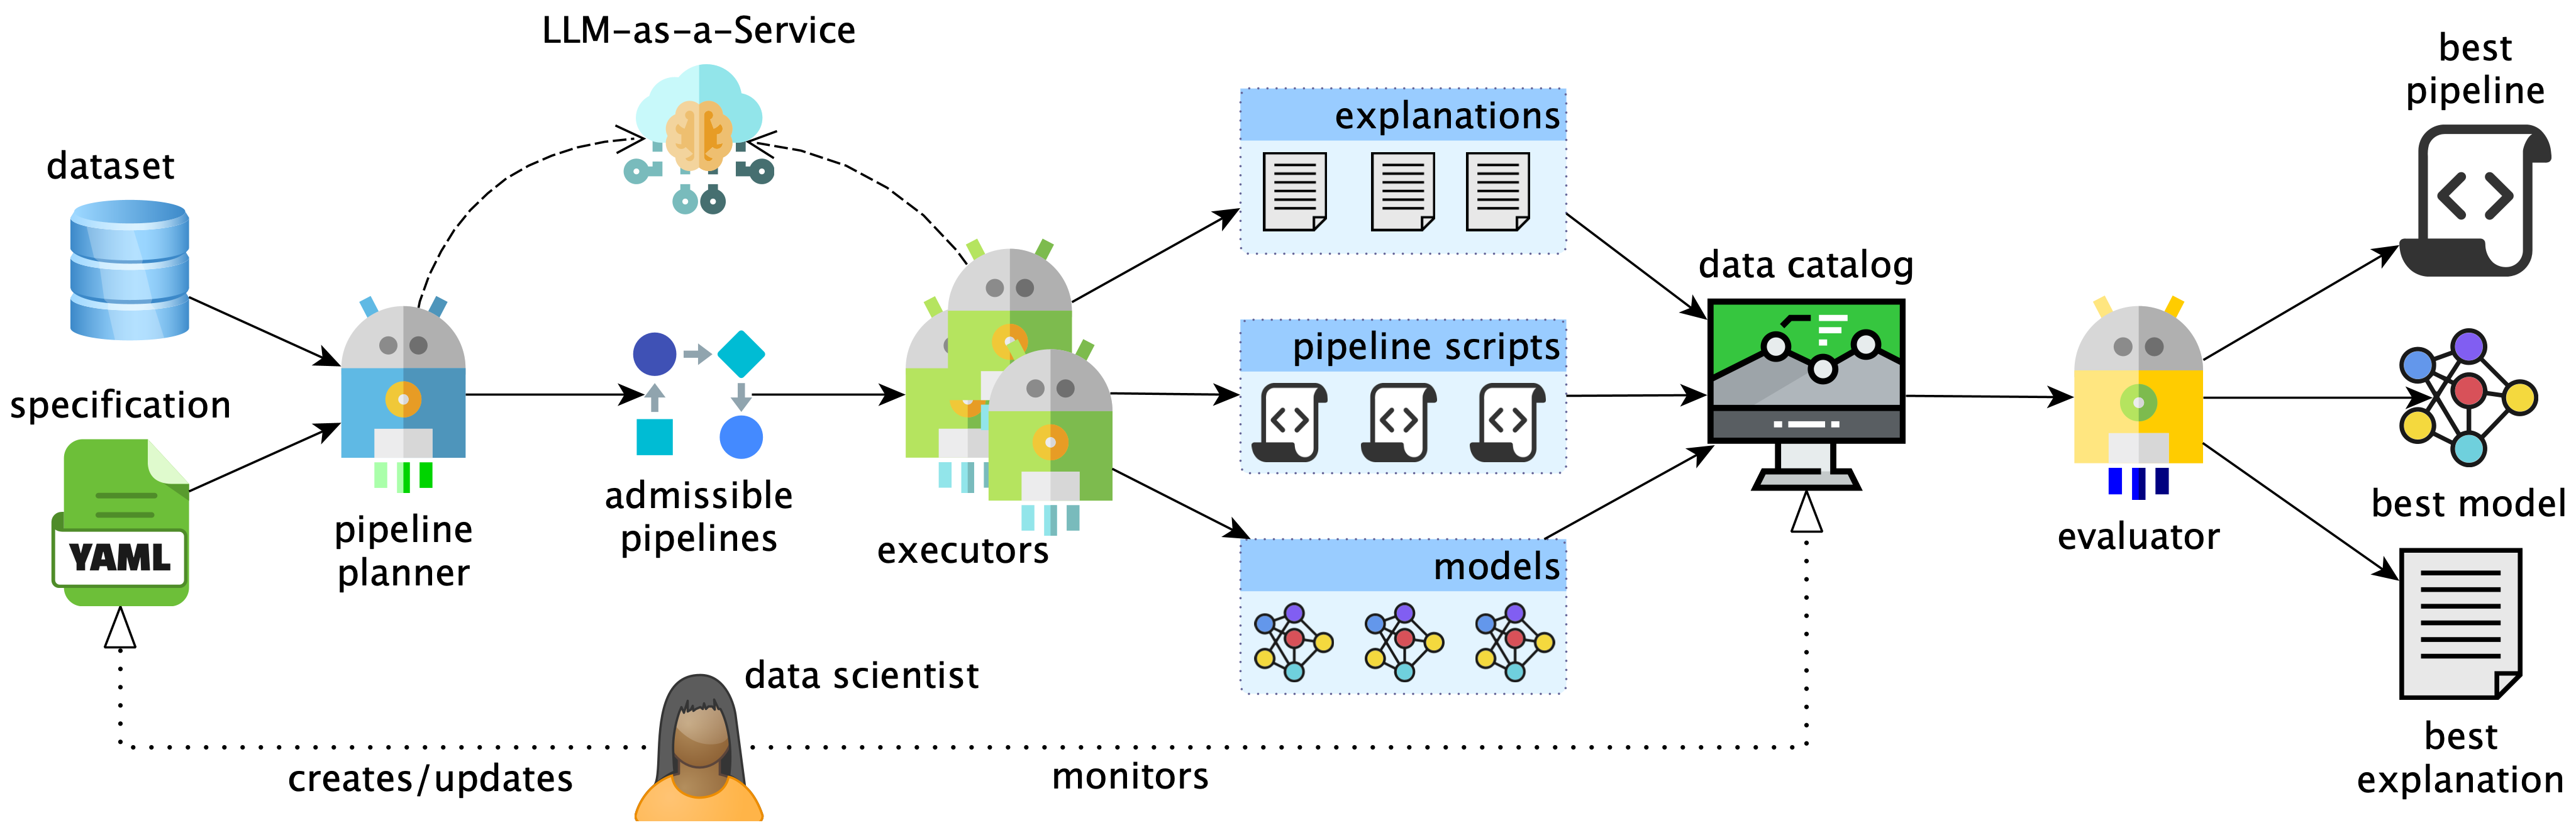
\includegraphics[width=\linewidth]{figures/agents-io.png}
  \caption{
    Overview of the agentic architecture for specification-driven \ac{AutoML}.
    Androids represent agents and dashed arrows denote interactions with \acp{LLM}.
  }
  \label{fig:layered-architecture}
\end{figure*}

\cref{fig:layered-architecture} shows the proposed architecture for specification-driven \ac{AutoML}.
%
The system consumes as input:
\begin{inlinelist}
  \item a dataset,
  \item a \textbf{specification}, % compliant with \cref{sec:specification-language},
  and
  \item a computational budget
\end{inlinelist}
and returns the best model found among the admissible pipelines.
%
Admissibility is determined by the data-science knowledge encoded in the specification,
whereas optimality is assessed empirically on the dataset at hand.
%
% Accordingly,
% the architecture addresses
% problem~\ref{prob:workflow-automation}
% by automating pipeline construction and execution,
% and problem~\ref{prob:explanation}
% by logging the decisions, scripts, metrics, and explanations produced during the process.
Additionally, the architecture consists of three agent types and one reactive component.
%
The \textbf{pipeline planner} agent parses the specification,
resolves dataset-dependent conditions,
and generates admissible pipeline plans.
%
The \textbf{pipeline executor} agent turns each plan into executable code,
runs it,
and stores the resulting artefacts.
%
The \textbf{data catalog} records execution traces,
including generated scripts,
hyper-parameters,
intermediate artefacts,
metrics,
and natural-language explanations.
%
Finally,
the \textbf{evaluator} agent compares the produced models on a held-out test set
and selects the best model,
together with its corresponding pipeline and explanation.
%
The planner and evaluator are singleton modules,
whereas executors can be instantiated in parallel,
thereby supporting budgeted exploration of multiple admissible pipelines.

\subsection{Specification}
\label{subsec:specification}

We adopt a YAML-like concrete syntax to keep specifications readable by practitioners,
parsable by software components,
and
amenable to \ac{LLM}-based generation and revision.
%
This kind of specification is inspired by SKI-Lang~\cite{skilang}
where YAML-like language is used to encode knowledge to be injected into a neural predictor.
%
The file comprises four main sections:
\texttt{pipeline},
\texttt{ordering},
\texttt{constraints},
and
\texttt{budgets}.
% \listingFromFile{yaml}{lst:spec-stub}{spec-stub.yml}{
%   Overall structure of the specification language, highlighting the main sections of a specification file.
% }
\listingFromFile{yaml}{lst:spec-ordering}{spec-ordering.yml}{
  Excerpt of specification.
}
\cref{lst:spec-ordering} shows an excerpt of specification.
\texttt{pipeline} specificies the admissible steps, their candidate implementations, and their hyper-parameter domains.
\texttt{ordering} specifies that the pipeline must first perform \textit{imputation} to handle missing data, then apply \textit{normalisation} to scale the features, and afterward execute the \textit{features} step for feature engineering or feature selection.
\texttt{constraints} states that when the classification algorithm is KNN, the pipeline must include both \textit{normalisation} and \textit{features} steps, since KNN is sensitive to feature scaling and often benefits from feature preparation.
Additionally, if the dataset contains a target feature whose name resembles \textit{class} or \textit{target} and whose data type is categorical or integer, then the pipeline must use \textit{classification}.
\texttt{budgets} defines execution budgets and resource limits for an automated search process, such as that at most 5 candidate pipelines may be evaluated and 10 number of attempts can be used to generate valid pipeline configurations.


\subsection{Pipeline planner}
\label{subsec:pipeline-planning}

Pipeline planning is the phase in which the system turns a specification into a set of admissible candidate pipelines.
%
Intuitively,
the planner agent reads the specification,
checks which rules apply to the input dataset,
and enumerates the pipelines that are compatible with the specification's constraints.
%
Most notably,
the planner agent samples the set of all admissible pipelines according to the budget constraints,
so the output of this agent is a \emph{subset} of the pipelines that satisfy the specification,
whose cardinality is determined by the \texttt{pipelines} budget.
%
Informally,
we refer to this set as the ``pipeline execution plan'',
because it contains the pipelines that will be executed in the next phases.

\subsubsection{Pipeline admissibility}
%
A pipeline is admissible when it is compatible with the data-science knowledge encoded in the specification:
it contains all mandatory steps,
respects the required ordering among steps,
and satisfies the declarative constraints relating dataset properties,
steps,
and candidate algorithms.
%
% For instance,
% a specification may require imputation whenever missing values are detected,
% normalisation before distance-based classifiers,
% or the exclusion of a candidate algorithm when its assumptions are violated.
%
The planner resolves these requirements before execution,
so that downstream only receive pipelines that are structurally valid with respect to the specification.

A pipeline can still be seen as a finite sequence of step--candidate pairs:
where each step denotes a phase of the workflow
and each candidate denotes the concrete algorithm or operation selected for that phase.
%
However,
the purpose of the planner is not to optimise hyper-parameters directly.
%
Rather,
it defines the admissible region of the workflow space:
which steps may appear,
in which order,
and with which candidate implementations.
%
Hyper-parameter optimisation is then delegated to pipeline executor agent.

\subsubsection{Finding admissible pipelines via \acs{CSP}}

The planner models ``admissibility'' as a finite-domain \ac{CSP}
tailored on the specification YAML file in input.
%
It then leverages a \ac{CSP} solver
-- currently, the Z3 theorem prover~\cite{DBLP:conf/tacas/MouraB08} --
to compute admissible pipelines efficiently.

The full \ac{CSP} model is reported in supplementary materials,
here we provide only an informal sketch of its main components and constraints.
%
For each possible step,
the \ac{CSP} records whether the step is selected,
where it appears in the pipeline,
and which candidate implements it.
%
The constraints ensure that:
%
\begin{inlinelist}
  \item every selected step has exactly one selected candidate;
  \item skipped steps have no candidate and no position in the pipeline;
  \item selected steps occupy distinct positions while being totally ordered
  \item mandatory steps are always selected;
  \item precedence relations from the specification among steps are respected;
  and
  \item declarative constraints from the specification are enforced,
  along with their require/forbid implications.
\end{inlinelist}
%
Thus,
constraints such as
``if the classifier is \texttt{knn}, then normalisation is required''
are compiled into logical constraints over the corresponding step and candidate variables.

% This modelling choice is useful for two reasons.
% %
% First,
% it makes the generation of pipelines \emph{sound} and \emph{complete}
% -- other than explicit and inspectable --:
% each solution of the \ac{CSP} corresponds to one admissible pipeline.
% %
% Second,
% it decouples validity from exploration.
% %
% The system can enumerate the whole admissible space when it is small enough,
% or sample from it when the number of solutions exceeds the available budget.
% %
% In the latter case,
% the computational budget determines how many admissible pipelines are selected for execution,
% while the \ac{CSP} guarantees that every sampled pipeline still satisfies the specification.
% %
% This is important because the budget constrains exploration,
% not correctness:
% budget limitations may prevent the system from trying all valid pipelines,
% but they should not cause invalid pipelines to be executed.

Once a satisfying assignment is obtained,
the planner reconstructs the corresponding pipeline by ordering the selected steps according to their assigned positions
and attaching to each step its selected candidate.
%
The resulting sequence is then passed to the pipeline executor,
which generates and runs the corresponding code.

% \paragraph{Dataset-related conditions, \acp{LLM}, and \acs{CSP}}

% Dataset-dependent constraints are especially relevant in our setting,
% because they are the point where the planner agent actively inspects the input data rather than merely compiling static rules.
% %
% When a constraint depends on the dataset,
% the planner agent queries an \ac{LLM} to decide whether the condition holds,
% possibly using dataset summaries,
% schema information,
% feature statistics,
% or small data samples as evidence.
% %
% For example,
% a specification may contain a rule such as (cf. \cref{lst:spec-constraints}):
% %
% \begin{quote}\itshape
%   if the input dataset has an \emph{output} feature named like ``class'' or ``target'' and that feature is categorical,
%   then classification step is \emph{required}
% \end{quote}
% %
% Before generating pipelines,
% the planner agent tests the antecedent of the rule on the concrete dataset.
% %
% If such a feature is detected,
% the rule is activated and only pipelines containing an imputation step are considered admissible.
% %
% Otherwise,
% the rule is ignored for that dataset.
% %
% Similarly,
% a rule may state that if numerical features have largely different scales,
% then normalisation should be required before distance-based classifiers such as \texttt{knn}.
% %
% In that case,
% the planner agent checks the dataset statistics,
% asks the \ac{LLM} to assess whether the scale mismatch is relevant,
% and then activates or deactivates the corresponding planning constraint.



\subsection{Pipeline executor}
\label{subsec:pipeline-execution}

\subsubsection{Code Generation}
% \malasidenote{si potrebbero rimuovere gli import per guadagnare spazio}

% Code generation is the process of translating an admissible pipeline
% produced by the planner into an executable and parametric Python script.
% %
% Executor agents are responsible for this process.

Code generation aims to bridge the gap between the symbolic representation of a pipeline
and a concrete training procedure that can be executed on actual data.
%
Given an admissible pipeline
the executor agent produces a Python program implementing exactly the candidate algorithms in the prescribed order,
without having to re-check admissibility,
% \malasidenote{in realtà c'è comunque lo step di validate\_code\_compliance}
which is already guaranteed by the pipeline planner.

The generated script is parametric with respect to the hyper-parameters
associated with the candidates appearing in the target pipeline in the user-provided specification.
%
The generated code exposes one parameter for each hyper-parameter,
so that the pipeline can be re-executed multiple times with different hyper-parameter values during the subsequent execution phase.

% \listingFromFile{python}{lst:generated-pipeline}{generated-pipeline.py}{
%   Generated code of a pipeline as a parametric Python function.
% }

% Operationally,
% the target artefact is a Python script,
% containing a function of the form
% \inlinePython{def train_model(X_train, y_train, ...)},
% where the additional arguments correspond to the selected hyper-parameters.
% %
% The function accepts a training set in input,
% constructs the corresponding \ac{ML} workflow,
% fits all intermediate components requiring training,
% and returns the trained model object,
% there including the fitted preprocessing and feature-engineering stages whenever present.
%
% An example of generated script is reported in \cref{lst:generated-pipeline},
% which shows a Python function implementing one admissible pipeline via \texttt{scikit-learn}.
%
% In particular,
% the function implements a pipeline with four steps:
% \texttt{normalisation},
% \texttt{features},
% \texttt{rebalancing},
% and
% \texttt{classification};
% corresponding to as many candidates, respectively:
% \texttt{MinMaxScaler},
% \texttt{SelectKBest},
% \texttt{NearMiss},
% and
% \texttt{MLPClassifier}.

\begin{figure}[t]
  \centering
  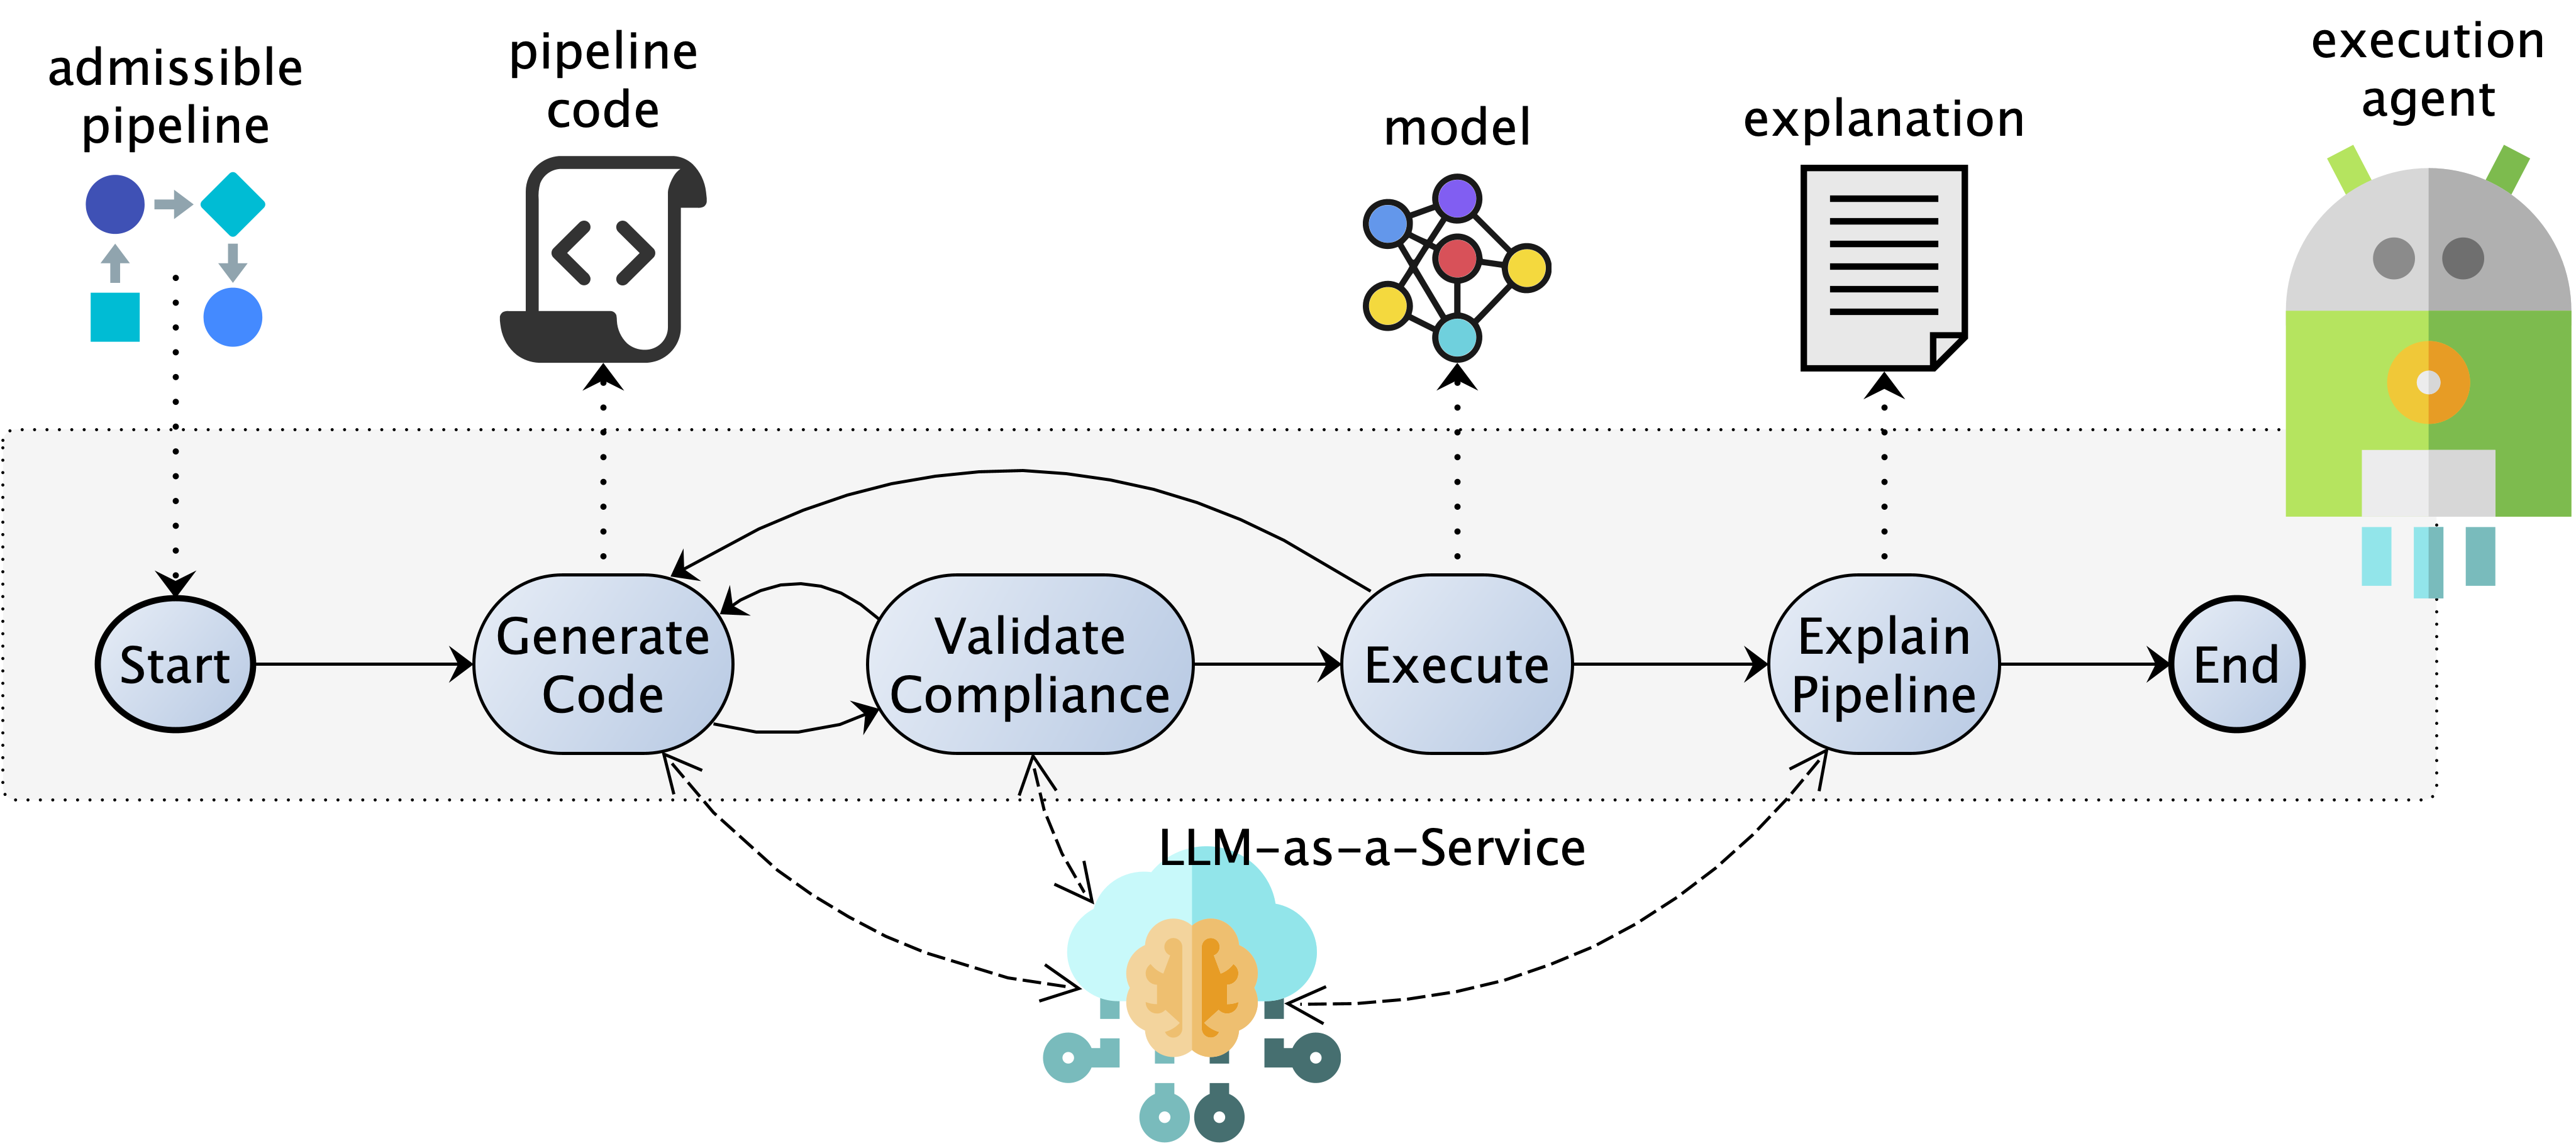
\includegraphics[width=\linewidth]{figures/executor-state-machine.png}
  \caption{
  State machine governing the behavior of executor agents.
    Starting from an admissible pipeline for the dataset at hand
    the agent iteratively generates Python code,
    validates its compliance w.r.t. the pipeline,
    executes it on the training set
    -- multiple times, exploring different hyper-parameter assignments --,
    and finally produces a textual explanation of outcome.
    % Dashed edges denote retry paths triggered by failed validation or failed execution.
  }
  \label{fig:executor-state-machine}
\end{figure}

\cref{fig:executor-state-machine} depicts the state machine governing behaviour of executor agents.
%
The figure highlights that code generation is not treated as a single-shot translation problem,
but rather as an iterative synthesis procedure in which generation,
semantic validation,
runtime validation,
and explanation are tightly coupled.
% 
The generation process starts by collecting the information needed to condition the synthesis task.
%
This includes:
\begin{inlinelist}
  \item a compact description of the dataset's structure,
  \item the parsed specification
  (which includes budget constraints,
  e.g. on the amount of retries allowed in the generation process,
  as well as token or time limitations),
  \item the admissible pipeline selected by the planner,
  \item the target feature,
  and
  \item the validation metric to be optimised.
\end{inlinelist}
%
Such information is used by executor agents to build the prompt context for some underlying \ac{LLM},
which is then asked to produce Python code,
with a fixed interface and responsibility.
%
% The interface is the aforementioned \texttt{train\_model} function,
% whose parameters include the training data and all hyper-parameters belonging to the selected candidates.
% %
% The responsibility is to implement all and only the steps occurring in the admissible pipeline,
% preserving their order.
%
% This design choice has two advantages.
% %
% First,
% it yields artefacts that are directly callable by executor agents.
% %
% Second,
% it decouples structural synthesis from hyper-parameter search:
% the code generation step produces one parametric script per admissible pipeline,
% whereas the executor later runs that script multiple times with different hyper-parameter assignments.

After code is generated,
executor agents perform an automatic validation step aimed at checking semantic compliance.
%
Rather than relying on syntactical correctness alone,
the generated program is inspected against the intended pipeline specification
to verify that it contains \emph{exactly} the expected steps and \emph{no unintended} ones.
%
This validation can be formulated as a combination of
\begin{inlinelist}
  \item a judgment problem in which a \ac{LLM} is asked to compare
  the admissible pipeline and the generated code,
  and determine whether the latter faithfully implements the former\footnotemark;
  and
  \item a matching problem in which the generated code matched against a number of regular expressions,
  to ensure that it matches the desired syntax,
  and that all necessary hyper-parameters are mentioned.
\end{inlinelist}
%
\footnotetext{
  In particular,
  the \ac{LLM}-as-a-judge approach is employed,
  to check that all necessary candidates appear in the code,
  and that no extraneous candidate is present.
}
%
Whenever any of these checks fail,
the feedback is injected back into the conversational context,
and a new generation attempt is performed,
up to reaching the retry limit.

% Successfully validated code is then executed by the executor agent
% (see next subsection)
% and,
% if execution fails at runtime,
% another generation round is attempted,
% in compliance with the retry budget.

\subsubsection{Pipeline execution}

Pipeline execution starts once an executor agent has successfully generated
and validated a parametric script for some admissible pipeline.
%
At this point,
the script is assumed to expose a fixed training interface,
as discussed above,
and to contain one parameter for each hyper-parameter associated with the candidates occurring in the pipeline.
%
The executor then attempts to run the script on the input dataset.
%
As shown in \cref{fig:executor-state-machine},
execution is still part of the agentic control loop:
runtime failures are not treated as terminal errors by default,
but as feedback for the executor agent.
%
Whenever execution fails,
the agent backtracks to the generation phase,
unless the retry budget has already been exhausted.
%
% Thus,
% generation and execution jointly implement a bounded retry loop,
% where the budget controls how many failed attempts may be tolerated before abandoning the pipeline.

% \paragraph{Test-set separation}
% \label{par:test-set-separation}
% Before any generated script is executed,
% the dataset is split into training and \emph{test} partitions.
% %
% This operation is performed once at the beginning of the execution phase,
% and the split ratio is provided as a configurable launch parameter.
% %
% All executions of all generated scripts are then trained on the same training partition.
% %
% The held-out test partition is not accessed by executor agents during training;
% it is instead reserved for the evaluator agent,
% which later compares the trained models under a common experimental protocol.
% %
% This design avoids incomparable evaluations across pipelines,
% because differences in the final scores can be attributed to the generated workflows
% and their hyper-parameter assignments,
% rather than to different train--test splits.

% \paragraph{Hyper-parameter exploration}
% For each admissible pipeline,
% execution consists of running the corresponding script under multiple hyper-parameter assignments.
% %
% Let
% $
%   \mathbf{p}
%   % =
%   % (s_1:c_1,\ldots,s_L:c_L)
% $
% be the pipeline implemented by the script,
% and let
% $
%   \mathcal{H}_{\mathbf{p}}
%   % =
%   % \bigcup_{\ell=1}^{L} \mathcal{H}_{c_\ell}
% $
% be the set of hyper-parameters exposed by the selected candidates.
% %
% For each hyper-parameter
% $h \in \mathcal{H}_{\mathbf{p}}$,
% the specification provides a finite domain $\Lambda_h$.
% %
% The executor therefore considers the Cartesian product
% %
% $
%   \Lambda_{\mathbf{p}}
%   =
%   \prod_{h \in \mathcal{H}_{\mathbf{p}}} \Lambda_h
% $
% %
% as the set of admissible hyper-parameter assignments for that pipeline.
% %
% Each element
% $\lambda_{\mathbf{p}} \in \Lambda_{\mathbf{p}}$
% corresponds to one actual execution of the generated script.
% %
% In other words,
% the code-generation phase produces one parametric implementation per pipeline,
% whereas the execution phase materialises that implementation into several trained models,
% one for each explored assignment of the involved hyper-parameters.

\paragraph{Parallelism}

The execution process is parallelised at the pipeline level.
%
Given the set of admissible pipelines selected by the planner,
the system spawns as many executor agents as the number of pipelines to be explored,
within the limits imposed by the computational budget.
%
Consequently,
code generation,
validation,
runtime repair,
and execution may proceed concurrently for different pipelines.
%
This form of parallelism is deliberately coarse-grained:
each executor agent is responsible for one admissible pipeline,
including all its hyper-parameter assignments,
while the global budget bounds the number of pipelines,
generation retries,
and executions that may be attempted.

\paragraph{Explanation generation}

% As the executor agent iteratively generates,
% validates,
% and
% executes code for a given pipeline,
% issues may arise at any stage of the process.
% %
% When this happens,
% if retries are still available,
% the executor agent may attempt to fix the issue by generating a new version of the code,
% possibly conditioned on the error message or the failed validation feedback.
% %
% Any successful execution of a pipeline is therefore the result of a sequence of generation attempts,
% some of which may have persuaded the agent to structure the code differently.

The executor finally produces a natural-language explanation
of the whole generation--validation--execution process.
%
In doing so,
the agent steers the \ac{LLM} to summarise whole conversational context,
including the initial pipeline specification,
the generated code,
the validation feedback (in case of failed validation),
the execution feedback (in case of failed execution),
and the variations across generation attempts.

% The outcome is a textual file,
% explaining the final pipeline and its code.
% %
% The shape of these explanations is mildly constrained,
% but it is forced to include:
% \begin{inlinelist}
%   \item a user-friendly description of the steps and candidates included in the pipeline,
%   \item the purpose of each step and candidate in the pipeline,
%   \item a description of the pathway towards the final code,
%   including a motivation for the current code organisation,
%   and a description of any problem that arose during generation and execution,
%   along with the corresponding solution.
% \end{inlinelist}

The supplementary materials include examples of generated explanations.

\subsection{Data Catalog}
\label{subsec:logging}

\begin{figure}[t]
  \centering
  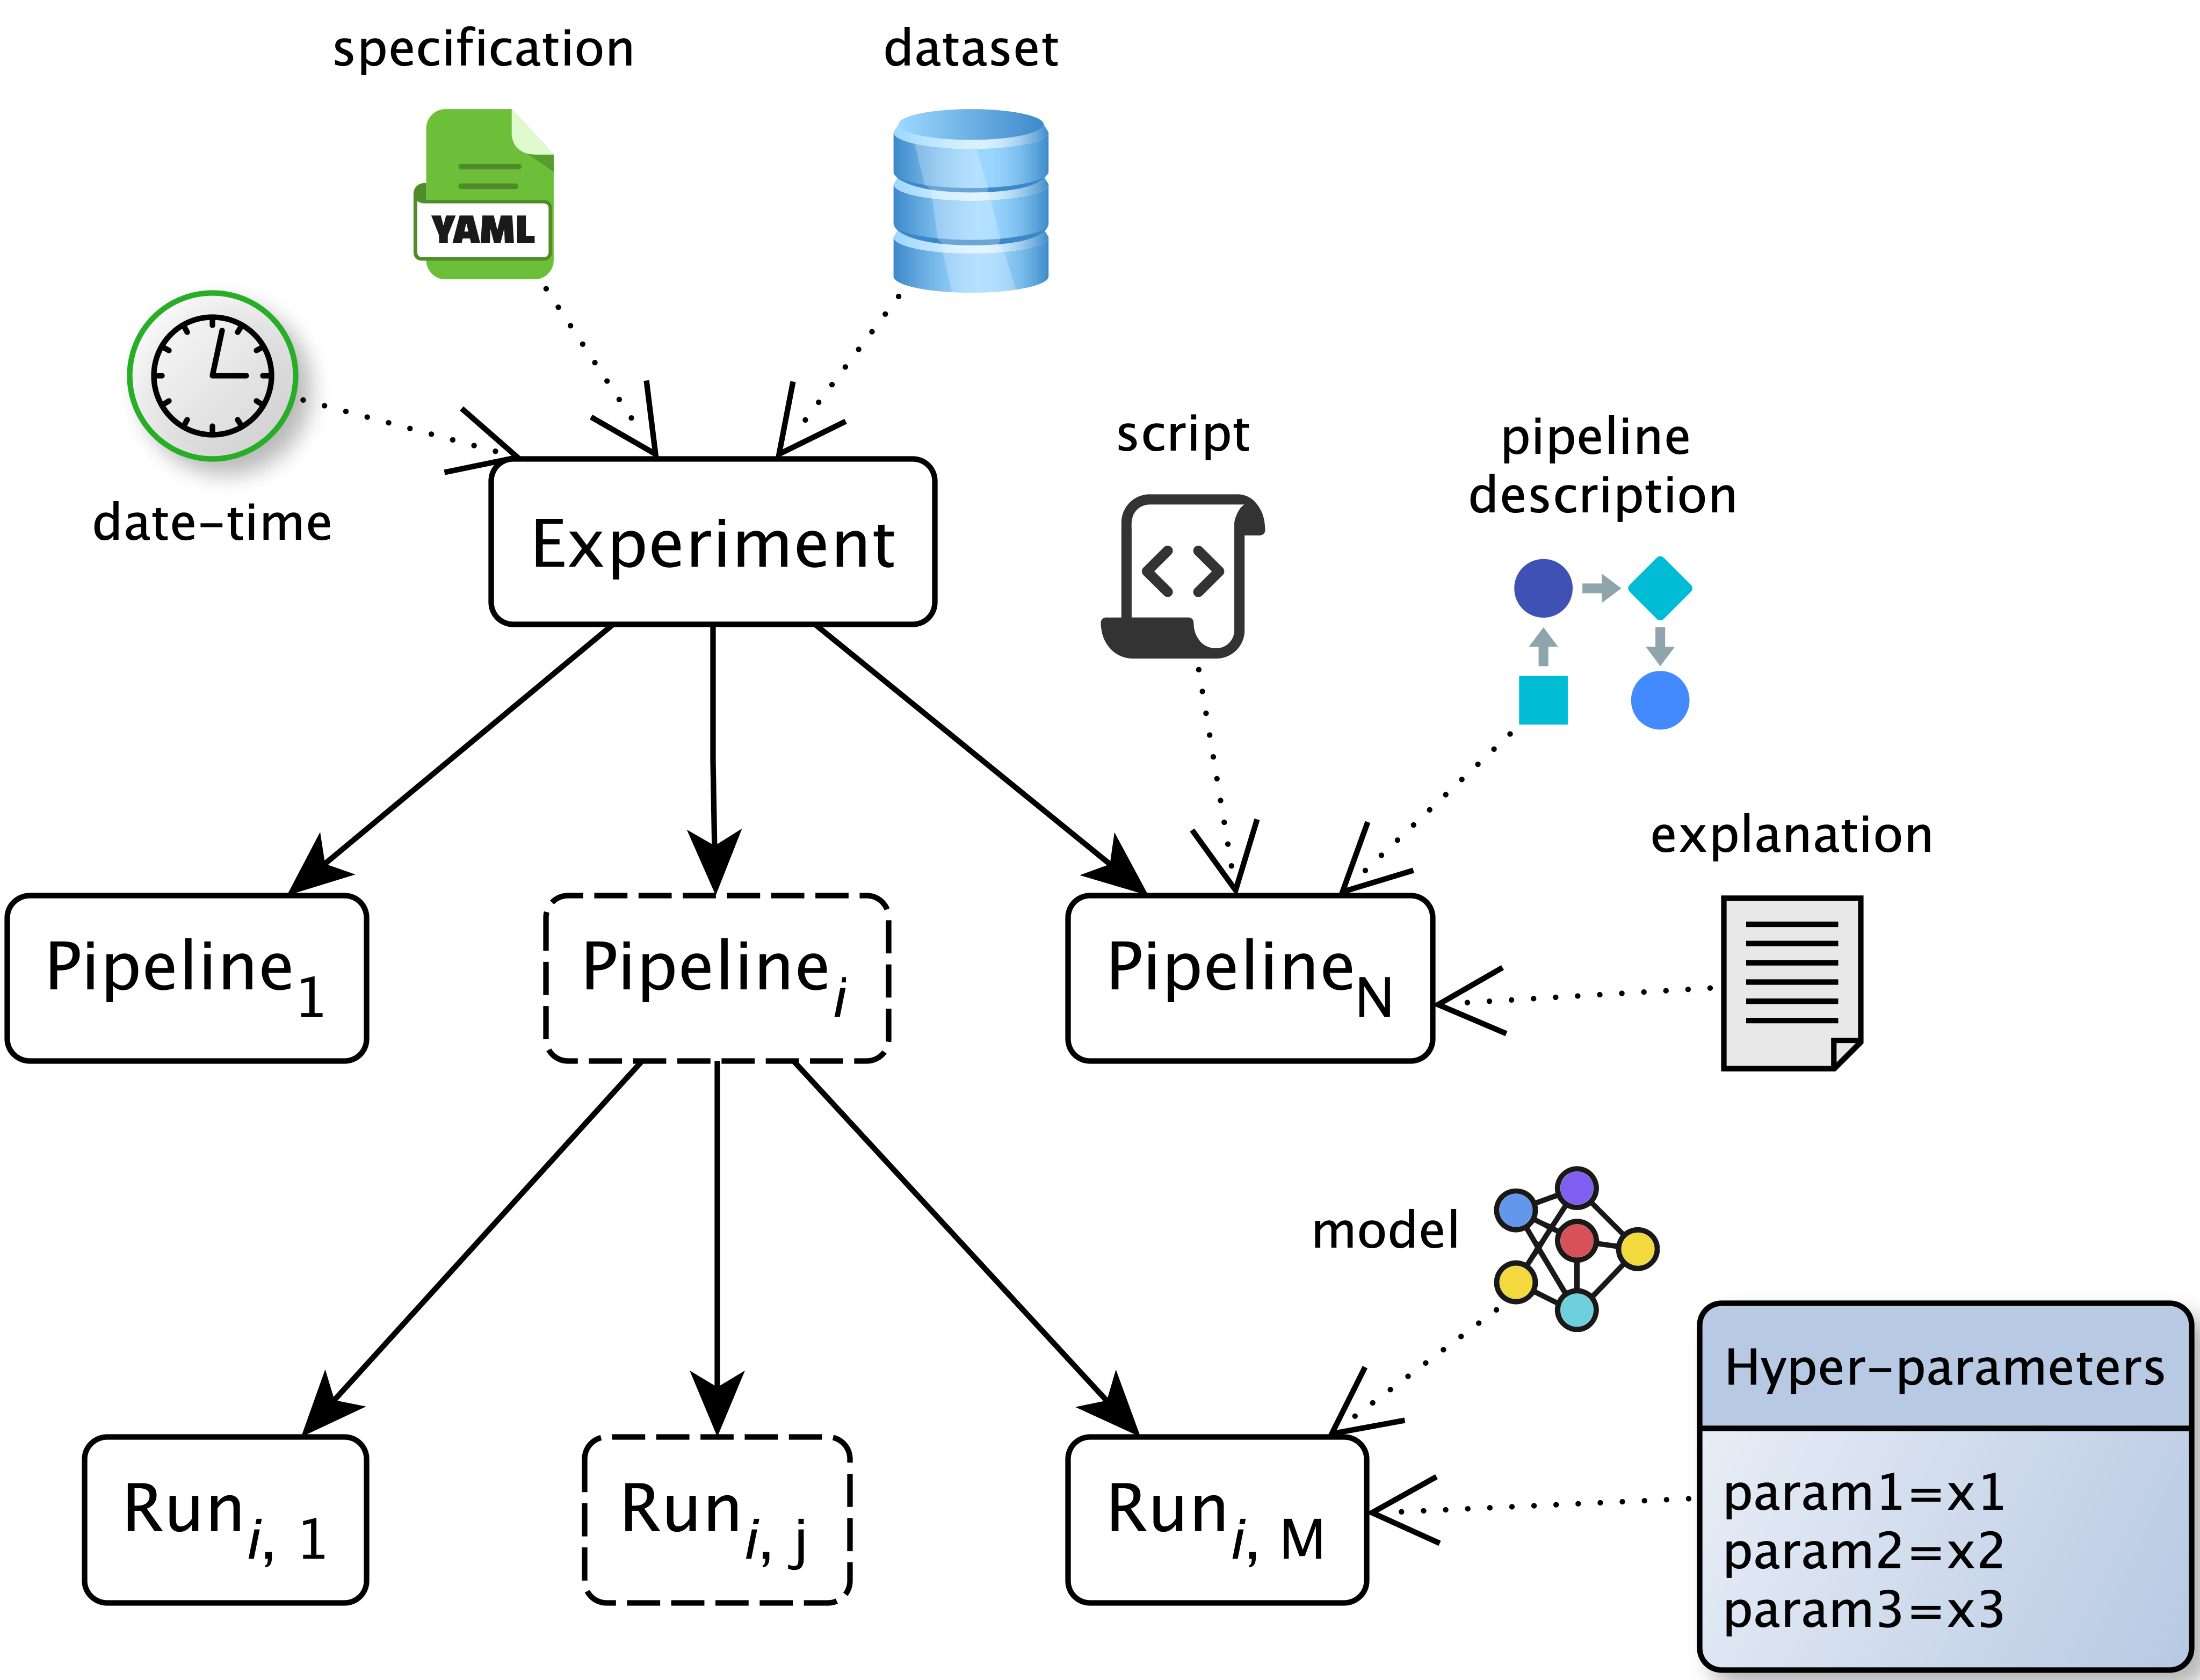
\includegraphics[width=\linewidth]{figures/hierarchy.png}
  \caption{
    Hierarchical logging scheme for the execution artefacts produced during specification-driven \ac{AutoML}.
    Dotted arrows denote metadata associations for entries at different levels of the hierarchy.
  }
  \label{fig:logging-hierarchy}
\end{figure}

All execution artefacts are tracked in the data catalog,
currently implemented with \texttt{MLflow}~\cite{zaharia2018accelerating},
in a hierarchical way\footnote{\texttt{MLflows} acts as a model/pipeline registry that treats AI models as cataloged assets with governed access, auditing, and lineage}.
%
The logged structure mirrors the 3-level hierarchy of the exploration process,
as shown in \cref{fig:logging-hierarchy}.
%
At the first level,
one experiment corresponds to the \ac{AutoML} problem instance,
namely:
user-provided specification plus input dataset;
%
possibly including metadata such as the date-time of execution.
%
At the second level,
there is one entry for each admissible pipeline selected by the planner.
%
Pipelines come with metadata involving their description
(steps and candidates),
as well as
their generated code and explanation.
%
At the third level,
there is one entry for each run of each pipeline script,
where metadata include hyper-parameter values,
trained model artefacts,
and their training statistics and performance.

This hierarchical logging scheme serves two purposes.
%
First,
it makes the exploration reproducible:
for each trained model,
one can recover the dataset split,
the generating script,
the pipeline structure,
the hyper-parameter assignment,
and the runtime trace that produced it.
%
Second,
it provides the evaluator agent with structured metadata organisation,
in order to simplify the identification of the best model,
as described in the next subsection.

\subsection{Evaluator}
\label{sec:evaluation-model-selection}

The evaluator agent is responsible for selecting the final model,
and therefore the best pipeline,
among those actually generated and executed by the executor agents.
%
This selection is empirical:
the chosen solution is the one that performs best
w.r.t. the runs completed for the current \ac{AutoML} problem instance%,
% rather than with respect to the entire space of theoretically admissible pipelines.
---in compliance with budget limitations.

To this end,
the evaluator traverses the aforementioned hierarchy of logged artefacts
(see \cref{fig:logging-hierarchy})
from the leaves to the root,
assessing the performance metrics of the trained models and propagating the best values up to the experiment level.
%
The particular performance metric to be optimised is specified as a launch parameter of the system.

% At the third level,
% % each logged entry corresponds to one concrete run of a generated pipeline script,
% % under a specific hyper-parameter assignment.
% % %
% the evaluator loads the trained model of each run,
% and computes its predictive performance on a validation set.
% %
% Such validation set is assumed to be split by executor agent,
% before any execution starts for the a given pipeline,
% by further splitting that pipeline's training data.
% %
% In this way,
% the evaluator can compare
% different runs of the same pipeline
% on the same pipeline-specific validation set.
% %
% The first step in this process,
% is therefore assessing the performance of all runs of a given pipeline,
% updating their third-level entries with the corresponding validation scores.

% The evaluator then aggregates performance results at the pipeline level,
% by identifying the best model among all runs of the same pipeline,
% and therefore the best run.
% %
% Accordingly,
% each second-level entry is enriched with summary metadata,
% including the identifier of the -- pipeline-wise -- best run,
% the associated best model and its hyper-parameters,
% and the achieved validation performance.

% Finally,
% for each second-level entry
% -- namely, for each admissible pipeline explored by the system --,
% the evaluator then identifies the (experiment-wise) best run among all pipeline-wise best ones.
% %
% To do so,
% it assesses these pipeline-wise best models on the held-out test set,
% which was separated initially
% (cf. \cref{par:test-set-separation}),
% and updates the metadata of the first-level experiment entry accordingly.

% This bottom-up update of the logging hierarchy makes model selection explicit and inspectable.
% %
% At the end of the process,
% the experiment-level entry contains the final outcome of the \ac{AutoML} process,
% % \malasidenote{falso, ma si può implementare}
% % GC: allora implementiamolo
% while pipeline-level entries preserve the best empirical configuration found for each explored workflow.
% %
% At the same time,
% all intermediate evaluations remain available in the data catalog
% for the sake of inspectability and human supervision.
% %
% The use of a backend equipped with a graphical interface
% -- such as \texttt{MLflow} in our implementation.%, as shown in \cref{fig:mlflow-nested-runs} --,
% therefore allows users not only to retrieve the automatically selected model,
% but also to inspect any intermediate model,
% compare alternative pipelines or hyper-parameter assignments,
% and manually override the automatic selection when domain-specific considerations suggest doing so.

% \begin{figure}[t]
%     \centering
%     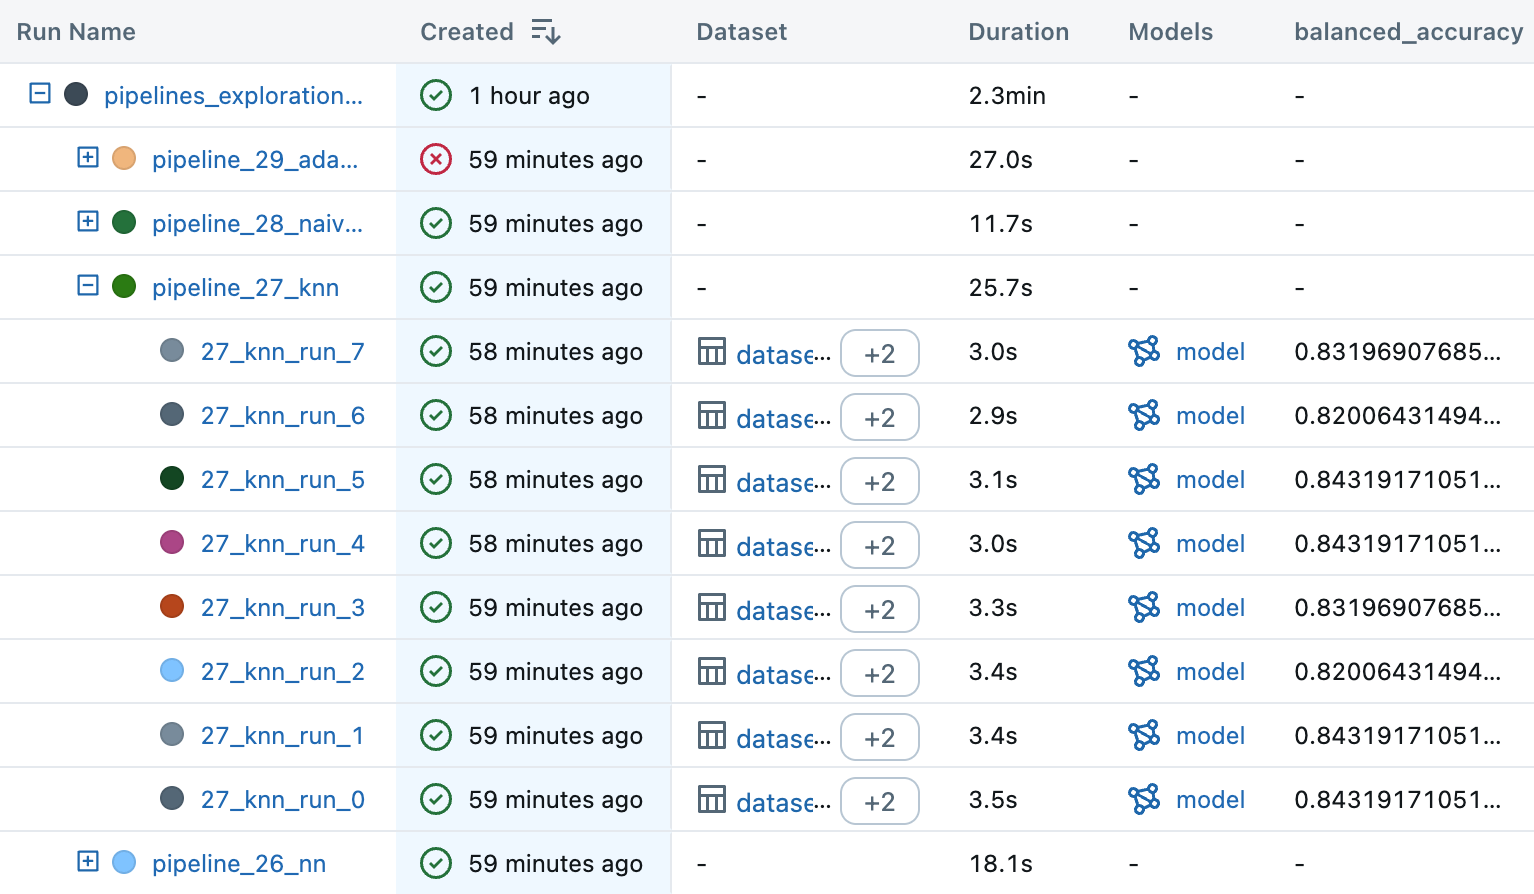
\includegraphics[width=\linewidth]{figures/mlflow/nested-runs.png}
%     \caption{
%         MLflow interface showing the hierarchical structure of nested runs with associated metadata.
%         At the top level, one experiment corresponds to one \ac{AutoML} problem instance.
%         At the second level, one entry corresponds to one admissible pipeline selected by the planner.
%         At the third level, one entry corresponds to one run of a generated pipeline script under a specific hyper-parameter assignment.
%     }
%     \label{fig:mlflow-nested-runs}
% \end{figure}

\section{Experimental Evaluation}
\label{sec:experimental-evaluation}

We empirically evaluate \ourapproach{} implementation,
both in \emph{absolute} terms
-- by assessing the predictive performance \ourapproach{} achieves on a collection of well-known benchmark datasets --,
and in \emph{relative} terms%
---by comparing the performance of \ourapproach{} against a state-of-the-art \ac{AutoML} system
(HAMLET~\cite{FranciaGP23}).

In particular,
\ourapproach{} consists of a Python system,
exploiting \texttt{LangChain}~\cite{Mavroudis2024}\footnote{\url{https://www.langchain.com}} and \texttt{LangGraph}\footnote{\url{https://www.langchain.com/langgraph}} for agent orchestration,
\texttt{Z3} for \ac{CSP} solving,
\texttt{MLflow} as the data catalog,
\texttt{scikit-learn} as the \ac{ML} library for generated pipelines,
and
of course our implementations of the pipeline planner, pipeline executor, and evaluator agents,
in compliance with the architecture from \cref{sec:agentic-architecture-for-specification-driven-automl}.
%
The source code of \ourapproach{},
along with automation scripts for reproducing our experiments,
are publicly available on GitHub\footnote{\label{url:repo}\url{https://github.com/Mala1180/age-ml}},
under an open-source license.

\paragraph{Experimental design}
\label{subsec:experimental-design}

% Our experimental evaluation is designed to assess the effectiveness of \ourapproach{} along two complementary axes:
% \begin{inlinelist}
%     \item predictive performance of the automatically generated machine learning pipelines, and
%     \item quality and utility of the explanations produced during the pipeline generation and execution process.
% \end{inlinelist}

% To this end, we define a single unified experimental setup applied consistently across all datasets described in \cref{subsubsec:datasets}.
%
% All experiments follow the same execution protocol and computational budget,
% while the analysis of results is subsequently decomposed into two distinct perspectives:
% performance analysis and explainability analysis.
%
The system is evaluated under a fixed computational budget defined in the experimental configuration, including:
a maximum of 30 pipelines to explore,
up to 8 parallel workers,
a maximum of 10 generation attempts per pipeline,
and a total time budget of 2 hours per run.
%
All executions are fully tracked using a data catalog (based on MLflow in the implementation),
enabling reproducibility and post-hoc analysis of both predictive outcomes and explanation artefacts.
Balanced accuracy is used for classification tasks and RMSE for regression tasks.

\paragraph{Datasets}
\label{subsubsec:datasets}

% !TEX root = paper-2026-agentic-automl.tex

\begin{table}[t]
    \centering
    \resizebox{\linewidth}{!}{
    \scriptsize
        \begin{tabular}{lcccccc}
        \hline
        Dataset & Problem & Features & Instances & Numeric & Discrete \\
        \hline
        Wilt & C & 5 & 4839 & 5 & 0 \\
        Texture & C & 40 & 5500 & 40 & 0 \\
        Madelon & C & 500 & 2600 & 500 & 0 \\
        HAR & C & 561 & 10299 & 561 & 0 \\
        Adult & C & 14 & 48842 & 6 & 8 \\
        MNIST\_784 & C & 784 & 70000 & 784 & 0 \\
        Ames Housing & R & 80 & 2930 & 37 & 43 \\
        California Housing & R & 8 & 20640 & 8 & 0 \\
        Auto MPG & R & 7 & 398 & 6 & 1 \\
        \hline
        \end{tabular}
    }
    \caption{
        Overview of the benchmark datasets used in the experimental evaluation.
        The datasets cover both classification (C) and regression (R).
        %tasks and include a diverse set of domains such as remote sensing, human activity recognition, image classification, tabular census data, and structured regression problems.
        %We report the total number of features, number of instances, and the breakdown between numerical and categorical attributes after preprocessing.
    }
    \label{tab:datasets}
\end{table}

We evaluate \ourapproach{} on a diverse collection of benchmark datasets commonly used in the machine learning literature,
covering both classification and regression tasks,
with varying dimensionality and feature types.
%
% The \textit{Wilt} dataset is a binary classification task derived from remote sensing data,
% where the objective is to distinguish diseased trees from healthy ones using spectral features extracted from satellite imagery.
% %
% The dataset is part of the UCI Machine Learning Repository collection of benchmark datasets and has been widely used in studies on imbalanced classification and remote sensing applications~\cite{dua2019uci}.
% It is relatively small and fully numerical.
%
% The \textit{Texture} dataset is a multiclass classification problem involving image texture recognition,
% where each instance corresponds to statistical descriptors extracted from texture images.
% %
% Texture representation and recognition have been extensively studied in the literature, for example using filter bank and texton-based representations~\cite{leung2001textons}.
% The dataset is moderately sized and entirely composed of numerical features.
%
% The \textit{Madelon} dataset is an artificial dataset designed specifically for feature selection benchmarking.
% It is a binary classification task with a high number of features, many of which are irrelevant or redundant,
% %
% making it particularly challenging for feature selection and model selection methods.
% It was introduced in the NIPS 2003 feature selection challenge~\cite{guyon2004nipsfs}.
%
% The \textit{\ac{HAR}} dataset consists of sensor signals collected from smartphones,
% used to classify different physical activities performed by subjects.
% %
% It is a multiclass classification problem with only numerical features.
% %
% The dataset was introduced for human activity recognition using smartphones~\cite{anguita2013har} and is used in wearable computing research.
%
% The \textit{Adult} dataset
% (also known as Census Income)
% is used for a binary classification task where the goal is to predict whether an individual's income exceeds a given threshold.
% %
% It contains a mix of numerical and categorical features and is one of the most widely used benchmarks for tabular classification.
% %
% It was introduced by Becker and Kohavi~\cite{becker1996adult}.
%
% The \textit{MNIST\_784} dataset is a well-known multiclass classification benchmark consisting of handwritten digit images.
% %
% Each instance is represented as a flattened vector of pixel intensities.
% %
% It originates from the work of LeCun et al.~\cite{lecun1998mnist} and remains a fundamental benchmark for image classification.
%
% The \textit{Ames Housing} dataset is for a regression problem aimed at predicting house prices based on a rich set of features describing residential properties.
% %
% It includes both numerical and categorical variables and is an extended and more modern alternative to the Boston Housing dataset~\cite{decock2011ames}.
%
% The \textit{California Housing} is a regression dataset where the goal is to predict median house values in California districts using demographic and geographic features.
% %
% It is derived from census data and is widely used for regression benchmarking~\cite{pace1997california}.
%
% The \textit{Auto MPG} dataset is used for a regression task focused on predicting fuel efficiency (miles per gallon) of automobiles based on various car attributes.
% %
% It contains both numerical and categorical features and was introduced by Quinlan~\cite{quinlan1993c45}.
%
\cref{tab:datasets} summarises the main characteristics of each dataset, including the number of instances, features, and the type of task.

\paragraph{Language models and prompts}
%
The experimental evaluation relies on \acp{LLM} to support code generation, validation, and explanation within the executor agents.
%
In particular,
we employ two models from the Gemini family,
namely \textit{Gemini 2.5 Flash} and \textit{Gemini 3.1 Flash Lite},
which are used across experiments without task-specific fine-tuning.
%
We deliberately choose small models to demonstrate that \ourapproach{} does not require large-scale \acp{LLM} to be effective,
and to keep the financial budget manageable.

Our agents interact with a small set of task-specific system prompts,
designed to enforce clear responsibilities.
%
In particular:
\begin{inlinelist}
  \item a code-generation prompt instructs the model to produce executable Python code implementing a given pipeline with a fixed interface,
  %
  \item a validation prompt frames the task as a compliance check between the intended pipeline and the generated code (LLM-as-a-judge), and
  %
  \item an explanation prompt requires the model to produce a structured,
human-readable description of the final pipeline and its design rationale.
\end{inlinelist}

Prompts are intentionally kept simple and consistent across experiments,
relying on the surrounding agentic loop to enforce correctness through iterative validation and feedback.
%
Full prompt definitions and implementation details are available on the repository\textsuperscript{\ref{url:repo}}
and in the supplementary materials.

% \subsection{Performance analysis}
% \label{subsec:performance-analysis}

% We evaluate \ourapproach{}'s ability to automatically construct high-quality machine learning pipelines starting from a general-purpose specification.
% %
% To do so,
% for each dataset,
% we let the system execute the full pipeline:
% \begin{inlinelist}
%   \item parsing of the specification and generation of admissible pipelines via the pipeline planner,
%   \item parallel execution of candidate pipelines,
%   \item hyperparameter exploration within each pipeline,
%   \item evaluation on a held-out test set (80--20\% split),
%   \item selection of the best-performing model.
% \end{inlinelist}
% %
% We then report the predictive performance on the test set,
% and the computational efficiency in terms of runtime and number of evaluated pipelines.

% \subsection{Explainability analysis}
% \label{subsec:explainability-analysis}
% %
% We also assess the quality and usefulness of the explanations generated by \ourapproach{} during pipeline construction and execution.
% %
% In particular,
% we assess whether the generated explanations:
% \begin{inlinelist}
%   \item correctly describe the sequence of transformations applied in the pipeline,
%   %
%   \item provide meaningful justification for model and preprocessing choices,
%   %
%   \item reflect constraint-driven decisions encoded in the specification, and
%   %
%   \item are informative enough to support human understanding and potential specification refinement.
% \end{inlinelist}

% For ease of analysis,
% we show one example of generated explanation for a successful pipeline.

\paragraph{Results}
\label{subsec:results}

\begin{table*}[ht!]
\centering
\small
\resizebox{\textwidth}{!}{%
\begin{tabular}{lrlccccrrrrr}
\hline
Dataset & Best Score & Baseline & Actual Time & Equivalent Time & LLM Inference Time & ML Training Time & Actual P. & Input Tokens & Output Tokens & Total Tokens & Putative Cost (\$) \\
\hline
Wilt & 0.983 & 0.975 & 0:03:24 & 0:24:34 & 0:14:40 & 0:09:54 & 30 & 615,707 & 33,780 & 649,487 & 0.614 \\
Texture & 0.992 & 0.997 & 0:03:13 & 0:28:06 & 0:16:58 & 0:11:08 & 30 & 2,017,288 & 35,480 & 2,052,768 & 1.208 \\
Madelon & 0.863 & 0.875 & 0:18:50 & 2:13:02 & 1:09:09 & 1:03:52 & 30 & 14,266,818 & 32,835 & 14,299,653 & 2.207 \\
HAR & 0.987 & 0.959 & 0:44:12 & 4:49:08 & 2:15:14 & 2:33:54 & 30 & 22,220,902 & 33,979 & 22,254,881 & 4.180 \\
Adult & 0.822 & 0.805 & 0:32:53 & 3:10:26 & 1:21:45 & 1:48:41 & 30 & 2,674,441 & 81,671 & 2,756,112 & 1.876 \\
MNIST\_784 & 0.971 & 0.972 & 2:00:28 & 7:03:17 & 2:54:24 & 4:08:52 & 25 & 17,785,846 & 27,616 & 17,813,462 & 5.615 \\
\hline
California Housing & 67,675.641 & 69,838.844 & 0:04:28 & 0:37:17 & 0:20:53 & 0:16:24 & 30 & 955,318 & 41,872 & 997,190 & 0.868 \\
Ames Housing & 30,189.152 & 29,660.363 & 0:03:49 & 0:29:23 & 0:20:22 & 0:09:01 & 29 & 4,071,760 & 65,523 & 4,137,283 & 2.017 \\
Auto MPG & 2.148 & 2.508 & 0:02:48 & 0:20:10 & 0:14:42 & 0:05:28 & 30 & 1,490,934 & 44,644 & 1,535,578 & 1.253 \\
\hline
\end{tabular}
}
\caption{Results obtained with Gemini 3.1 Flash Lite. Balanced accuracy is used for classification tasks (first six) and RMSE for regression tasks (last three). Values in bold indicate better performance than the baseline. Actual P. stands for the actual number of pipelines correctly executed (out of the budget of 30). }
\label{tab:gemini_3_1_flash_lite_results}
\end{table*}
\begin{table*}[t]
\centering
\footnotesize
\resizebox{\textwidth}{!}{%
\begin{tabular}{lccccccc}
\hline
Dataset & \ourapproach{} & Baseline & Actual P. & Input Tokens & Output Tokens & Total Tokens & Putative Cost (\$) \\
\hline
Wilt & 0.966 & 0.975 & 30 & 413,432 & 119,853 & 533,285 & 0.656 \\
Texture & 0.995 & 0.997 & 30 & 1,645,606 & 135,529 & 1,781,135 & 1.075 \\
Madelon & 0.863 & 0.875 & 18 & 7,368,780 & 80,067 & 7,448,847 & 1.855 \\
HAR & \textbf{0.981} & 0.959 & 12 & 8,305,395 & 66,378 & 8,371,773 & 2.864 \\
Adult & \textbf{0.813} & 0.805 & 30 & 3,533,767 & 864,794 & 4,398,561 & 3.933 \\
MNIST\_784 & 0.966 & 0.972 & 11 & 5,932,213 & 47,113 & 5,979,326 & 1.610 \\
\hline
California Housing & \textbf{69,331.032} & 69,838.844 & 30 & 1,620,167 & 492,151 & 2,112,318 & 2.258 \\
Ames Housing & 31,970.630 & 29,660.363 & 30 & 4,504,694 & 640,509 & 5,145,203 & 3.431 \\
Auto MPG & \textbf{2.283} & 2.508 & 30 & 1,662,359 & 244,199 & 1,906,558 & 1.694 \\
\hline
\end{tabular}
}
\caption{Results obtained with Gemini 2.5 Flash.}
\label{tab:gemini_2_5_flash_results}
\end{table*}

% \begin{figure}[t]
%     \centering

%     \begin{subfigure}{.49\linewidth}
%         \centering
%         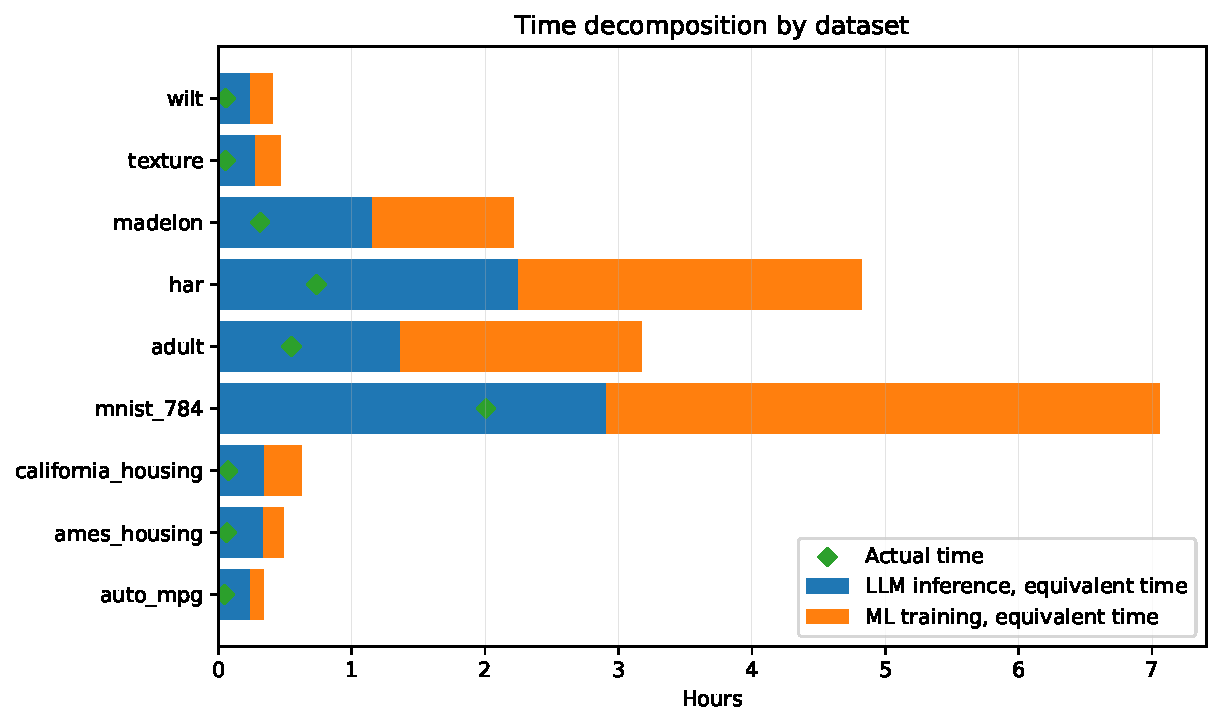
\includegraphics[width=\linewidth]{figures/gemini-3_1-flash-lite/04_time_breakdown}
%         \caption{\textit{Gemini 3.1 Flash Lite}}
%         \label{fig:gemini-3_1-flash-lite-time-breakdown}
%     \end{subfigure}
%     \begin{subfigure}{.49\linewidth}
%         \centering
%         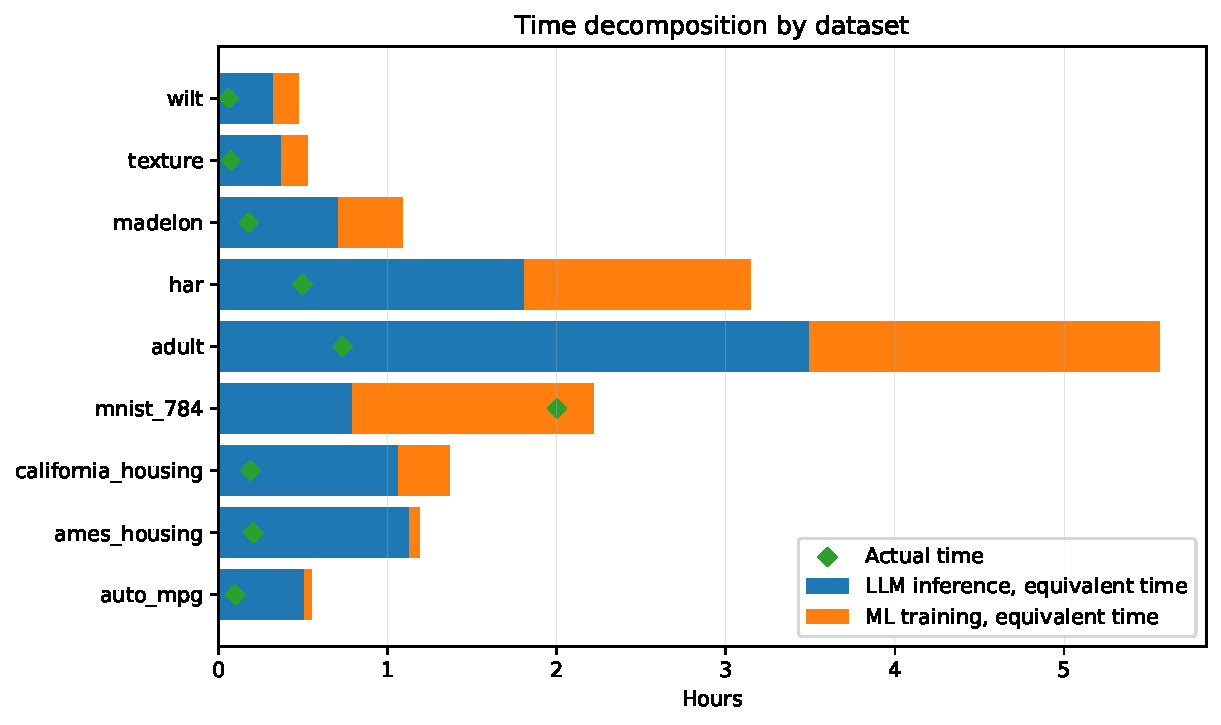
\includegraphics[width=\linewidth]{figures/gemini-2_5-flash/04_time_breakdown}
%         \caption{\textit{Gemini 2.5 Flash}}
%         \label{fig:gemini-2_5-flash-time-breakdown}
%     \end{subfigure}

%     \caption{Time breakdown across datasets.}
%     \label{fig:gemini-time-breakdown}
% \end{figure}

\cref{tab:gemini_3_1_flash_lite_results,tab:gemini_2_5_flash_results} report
the results obtained with \textit{Gemini 3.1 Flash Lite} and \textit{Gemini 2.5 Flash},
respectively,
across the six classification and three regression datasets.
%
%For the baseline,
%we report the performance of HAMLET~\cite{FranciaGP23} for classification
%-- except for \textit{MNIST\_784},
%where we report the performance of Hyperopt-sklearn~\cite{DBLP:books/sp/19/FeurerKES0H19} --
%and notebooks from Kaggle for regression.
%\gcsidenote{Bisogna dire perchè questo trattamento diverso per alcuni dataset}
For the baseline,
we use the performance of HAMLET~\cite{FranciaGP23} or Kaggle notebooks (where HAMLET is not available).
%
In particular,
for \textit{Ames Housing},
we consider Gus Martins' results%
\footnote{\url{https://www.kaggle.com/code/gusthema/house-prices-prediction-using-tfdf}},
for Auto MPG we use Ertu\u{g}rul Demir's work%
\footnote{\url{https://www.kaggle.com/code/datafan07/auto-mpg-eda-feature-engineering-and-regressions/notebook}},
for California Housing we report Ahmed Mahmoud's notebook%
\footnote{\url{https://www.kaggle.com/code/ahmedmahmoud16/california-housing-prices}}.

Both models generate pipelines that achieve competitive performance with respect to the baselines,
often matching or surpassing them despite operating under a constrained computational budget and without task-specific tuning.
%
Across classification tasks,
\textit{Gemini 3.1 Flash Lite} outperforms the baseline in 3 out of 6 datasets (\textit{Wilt}, \textit{HAR}, \textit{Adult}),
matches or remains close in others,
and shows only marginal degradation on more challenging benchmarks such as \textit{Madelon} and \textit{MNIST\_784}.
%
Similarly,
\textit{Gemini 2.5 Flash} achieves improvements over the baseline in 2 out of 6 datasets,
while remaining competitive in the remaining cases.
%
On regression tasks, both models demonstrate strong performance.
\textit{Gemini 3.1 Flash Lite} improves over the baseline in 2 out of 3 datasets (\textit{California Housing} and \textit{Auto MPG}),
while \textit{Gemini 2.5 Flash} also achieves improvements in 2 out of 3 datasets,
although with slightly higher variance and a more noticeable degradation on \textit{Ames Housing}.

A key difference between the two models lies in their ability to explore the search space.
%
\textit{Gemini 3.1 Flash Lite} consistently executes the full pipeline budget
(30 pipelines in almost all datasets),
whereas \textit{Gemini 2.5 Flash} often fails to reach the maximum number of valid pipelines
(e.g., 12 on \textit{HAR} and 11 on \textit{MNIST\_784}).
%
This reduced exploration might directly impact performance,
particularly on more complex datasets.

From an efficiency perspective,
the two models exhibit distinct computational profiles.
%
\textit{Gemini 3.1 Flash Lite} shows a more balanced distribution between \ac{LLM} inference and ML training time,
while \textit{Gemini 2.5 Flash} tends to spend a significantly larger fraction of time in inference
(e.g., more than 70\% of the total time on \textit{Adult} and \textit{California Housing}).
%
This suggests that the former achieves a more effective integration between the agentic loop and the underlying \ac{AutoML} components.
%
% \cref{fig:gemini-time-breakdown} provides a detailed breakdown of the runtime for both models across datasets,
% highlighting the differences in their computational profiles.

Token consumption further highlights this trade-off.
%
While \textit{Gemini 3.1 Flash Lite} generally uses more input tokens due to broader exploration,
\textit{Gemini 2.5 Flash} produces substantially more output tokens, indicating longer or less concise generations.
%
This results in comparable or higher overall costs for \textit{Gemini 2.5 Flash} despite exploring fewer pipelines.

% A qualitative inspection of the generated pipelines confirms that the system constructs semantically coherent and non-trivial workflows.
% %
% For instance,
% on the \textit{Adult} dataset,
% the best-performing pipeline integrates imputation, normalisation, feature selection, class rebalancing via SMOTE, and a neural classifier.
% %
% Importantly,
% such pipelines are not generated in a single step but emerge through iterative refinement,
% where issues such as categorical feature handling and label encoding inconsistencies are progressively resolved.
% %
% The full explanation is reported in supplementary materials.

% Overall,
% these results demonstrate that the proposed framework is capable of autonomously generating competitive machine learning pipelines,
% while effectively balancing exploration, computational efficiency,
% and correctness through the agentic loop.

\paragraph{Discussion}

The results show that the proposed approach generalises well across heterogeneous datasets,
including low-dimensional tabular data,
high-dimensional feature selection benchmarks,
and moderately complex image-derived representations.
%
Performance gains are particularly evident in scenarios requiring coordinated preprocessing steps
(e.g., \textit{Adult} and \textit{HAR}),
where the agentic loop successfully composes multiple transformations.
%
% In contrast,
% slightly weaker performance on datasets such as \textit{Madelon} and \textit{MNIST\_784}
% suggests that purely structural search may be insufficient when strong inductive biases or specialised model architectures are required.
% 
An important factor affecting performance is the number of successfully executed pipelines.
%
Datasets where fewer valid pipelines are generated
(e.g., \textit{HAR} and \textit{MNIST\_784} with \textit{Gemini 2.5 Flash})
exhibit lower performance,
indicating that pipeline validity and executability are critical bottlenecks in LLM-driven \ac{AutoML}.
%
This highlights the importance of the validation loop not only as a correctness mechanism,
but also as a key enabler of effective search.

% \subsection{Limitations and risks}

% Despite the promising results, several limitations must be acknowledged.
% %
% The framework heavily relies on the correctness and consistency of \acp{LLM}.
% %
% Errors in code generation, hallucinated \acp{API}, or inconsistent reasoning can negatively affect pipeline validity and performance.
% %
% While the validation loop mitigates some of these issues,
% it does not fully eliminate them, especially under strict time or budget constraints.
% %
% Choosing a capable model is crucial to ensure that the system can effectively explore the search space and generate valid pipelines.

% The agentic loop involves multiple interactions with \acp{LLM},
% including generation, validation, and explanation.
% %
% This results in non-negligible computational and monetary costs,
% particularly when exploring large search spaces or using more capable models.
% %
% Based on the budget at disposal,
% one can trade-off the time and the number of pipelines with the choice of a more or less capable \ac{LLM}.

% Due to the stochastic nature of \acp{LLM},
% and the sampling of just a portion of all the possible pipelines,
% repeated executions may lead to different pipelines and results,
% even under the same configuration.
% %
% While experiment tracking mitigates this issue, it does not fully guarantee determinism.



\section{Conclusion and Future Work}
\label{sec:conclusion}

This paper presents \ourapproach{}:
an agentic \ac{AutoML} approach focused on explainable, data-centric process automation from an \ac{MLOps} perspective.
%
\ourapproach{} enables practitioners to guide pipeline exploration through a high-level specification language designed to express custom constraints and \ac{ML} best practices.
%
Given time and cost budgets,
the system explores the space of admissible pipelines defined by the specification to identify high-performing solutions for the target task.
%
Experiments show that \ourapproach{} can generate competitive pipelines across heterogeneous datasets,
while providing meaningful explanations and a transparent optimisation process.

The main contributions of this work are:
%
\begin{inlinelist}
\item a specification language for data-centric \ac{AutoML} pipeline exploration,
\item symbolic enumeration of feasible pipelines,
\item automated code generation and execution,
and
\item logging of runs, artefacts, results, and explanations.
\end{inlinelist}


Future work will address several directions to enhance the system's capabilities and applicability.

\begin{itemize}
\item Enhancing the process of writing specification files by introducing agents capable of generating specifications from natural-language sources such as documentation, web resources, and expert comments.
This would improve accessibility for non-experts and reduce effort for experienced practitioners.
\item Introducing support for directly editing generated pipelines and selectively re-executing only modified components.
Adding this feature would provide greater human involvement and iterative refinement during model selection.
\item Investigating more efficient heuristic-based search strategies to improve exploration diversity.
\item Extending evaluation across multiple \acp{LLM}, since the architecture already supports easy integration of new providers but the current evaluation relies on a single provider (Google) and a limited set of models.
\item Optimising token usage by redesigning prompts and reducing redundant conversational context, while preserving pipeline quality.
\end{itemize}



\section*{Acknowledgement}

Matteo Magnini was supported by the Luxembourg National Research Fund (FNR)
through the project ``A DJ for Machine Ethics: the Dialogue Jiminy'' (O24/18989918/DJ4ME).

Experiments have been enabled by our friend and colleague Dr.\ Gianluca Aguzzi
(currently employed at the Università di Bologna),
who kindly provided us with access to his credit for \acp{LLM} usage on Google AI studio,
as provided by his Gemma Academic Program Award 2025.
%Experiments have been enabled by our friend and colleague Dr.\ Gianluca Aguzzi
%(currently employed at the Università di Bologna),
%who kindly provided us with access to his credit for \acp{LLM} usage on Google AI studio,
%as provided by his Gemma Academic Program Award 2025.

\bibliography{bibliography}
\bibliographystyle{splncs04}
\end{document}


